\documentclass[journal]{IEEEtran}

\usepackage{amsmath,amsfonts,amssymb}
\usepackage{algorithm}
\usepackage{algpseudocode}
\usepackage{array}
\usepackage[caption=false,font=normalsize,labelfont=sf,textfont=sf]{subfig}
\usepackage{textcomp}
\usepackage{stfloats}
\usepackage{url}
\usepackage{graphicx}
\usepackage{cite}
\usepackage{booktabs}


\hyphenation{op-tical net-works semi-conduc-tor IEEE-Xplore}

% \checkmark is an amssymb *math* symbol; \ensuremath keeps it legal in table
% cells and in a caption, where bare use would raise "Missing $ inserted".
\newcommand{\yes}{\ensuremath{\checkmark}}
\newcommand{\no}{---}

\begin{document}

\title{Trigger-Agnostic Behavioral Trust for Backdoor-Resilient\\ Federated GPS Spoofing Detection in UAV Networks}

\author{
Will~Jedrzejczak,
Cole~Walther,
Dilpreet~Gill
\thanks{Department of Computer Science, James Madison University. Advisor: Dr. Khalid Hasan.}
}

\maketitle

\begin{abstract}
Federated learning (FL) lets a fleet of unmanned aerial vehicles (UAVs)
train a shared GPS spoofing detector without raw receiver measurements
leaving any aircraft. Existing FL detection frameworks for UAV networks
assume honest participation, and several weight each client's
contribution by the validation accuracy that client reports about
itself. We show that this assumption is exploitable. We construct a
stealthy backdoor in which two of ten UAV clients poison part of their
local data using a trigger drawn from within the benign distribution,
scale their updates so the poison survives averaging, and inflate their
reported accuracy to obtain disproportionate aggregation weight. Across
three independent runs the attack raises backdoor success by $0.2415$
over the honest baseline while clean accuracy falls by less than two
points, and accuracy inflation raises it further to $0.3036$, making the
weighted rule worse than no weighting at all. We then
propose a defense in which the coordinator judges each client only by
behavior it observes on a small held-out root set, never reading
reported accuracy, which renders inflation inert by construction. Rather
than probing a designated trigger feature, the coordinator probes every
discriminative feature on counterfactual spoofed samples and scores each
client by its worst deviation below the cohort median in median absolute
deviations, then applies the resulting trust weights ahead of
coordinate-wise median aggregation. Under independent and identically
distributed clients the defense reduces attack-induced backdoor lift to a
level statistically indistinguishable from the honest baseline (lift
$-0.0265 \pm 0.0174$), flags both compromised clients in 100\% of
client-rounds at a 0.3\% honest false-flag rate, generalizes to trigger
features it was never given, remains effective against the tested
defense-aware evasion objective, and adds 34.0~ms of measured server-side
computation per round in the evaluated ten-client configuration, with no
additional client-side work. We compare against eight published
aggregation rules reimplemented on the identical pipeline. FLTrust, the
closest prior root-of-trust defense, leaves $+0.0787$ of lift and costs
utility relative to the honest baseline; Multi-Krum is competitive with
our behavioral trust under IID clients, a result we report rather than
obscure. What distinguishes the behavioral probe is that it needs no
estimate of how many clients are compromised, a condition under which
Multi-Krum degrades from $+0.0061$ to $+0.2837$, and that it names the
compromised aircraft rather than only excluding updates. We also report
the defense's principal failure: under client class-ratio skew the probe
stops firing, because suspicion measured against a cohort median is
masked by the honest cohort's own inflated variance, leaving the
coordinate-wise median backstop to carry what protection remains. All
results are obtained on a public software-defined-radio GPS spoofing
dataset partitioned into simulated UAV clients.
\end{abstract}

\begin{IEEEkeywords}
Federated learning, UAV networks, wireless security, backdoor attack, model poisoning, robust aggregation, behavioral trust.
\end{IEEEkeywords}

\section{Introduction}
\IEEEPARstart{U}{\textnormal{nmanned}} aerial vehicles (UAVs) increasingly depend on wireless navigation and communication links to carry out coordinated missions such as disaster response, infrastructure inspection, and search and rescue \cite{mekdad2023survey}. Because these links are openly broadcast over radio frequencies, they are exposed to a well-documented class of attacks, including GPS spoofing, that can degrade or hijack a UAV's perceived position without requiring any physical access to the vehicle \cite{mekdad2023survey}, \cite{chai2025navigation}. A single successful attack against even one node in a UAV fleet can cascade into mission failure, making early and reliable detection a safety-critical requirement rather than a convenience.

Detecting these attacks has historically relied on centralized approaches, in which raw navigation and sensor telemetry from every UAV is transmitted to a ground station or cloud server for analysis. This design is increasingly viewed as impractical for fleet-scale deployment: it concentrates sensitive operational data in one location, introduces a single point of failure, and is bandwidth-prohibitive precisely when the wireless channel is already degraded by an active attack \cite{udin2025federated}. Federated learning (FL) has emerged as a response to these limitations \cite{mcmahan2017communication}. Rather than sharing raw data, each UAV trains a local detection model on its own observations and shares only model parameter updates with a central aggregator, which combines them into an improved global model \cite{chai2025navigation}, \cite{udin2025federated}.

Recent work has applied FL specifically to UAV and FANET attack detection, and this body of work can be grouped by what it optimizes for and what it leaves unexamined. A first group focuses on improving raw detection accuracy under benign or randomly noisy client conditions. Mowla et al. propose an on-device FL architecture for jamming detection in flying ad-hoc networks (FANETs) with a client-group prioritization mechanism, but assume all participating UAV clients report honestly and do not consider an adversarial client manipulating its own contribution \cite{mowla2020federated}. Chai et al. propose a TCN-Transformer architecture trained via FL across distributed nodes, and introduce an accuracy-weighted aggregation strategy that dynamically assigns each client a weight based on that client's own detection performance, explicitly to reward high-quality contributions; their evaluation, however, assumes this reported performance is truthful and does not consider a client that misreports it \cite{chai2025navigation}. Ud Din et al. similarly propose a trust-weighted FL framework for UAV-enabled IoT networks, incorporating behavioral consistency and contribution-frequency metrics into the aggregation process, but likewise do not model a client that deliberately falsifies the metrics feeding its own trust score \cite{udin2025federated}. All three works report that performance- or trust-weighted aggregation outperforms standard federated averaging (FedAvg) under realistic UAV conditions, but none evaluates this advantage under an actively adversarial client.

A second group studies FL security in general, independent of the UAV setting, and establishes that aggregation itself is a viable attack surface. Bagdasaryan et al. show that a single compromised participant can use model replacement to implant a hidden backdoor into a federated model that performs normally on the main task while secretly misclassifying an attacker-chosen trigger pattern, but their attack and evaluation target plain FedAvg with uniform or data-proportional client weights, not an aggregation rule that weights clients by a self-reported, unverified metric \cite{bagdasaryan2020backdoor}. Fang et al. demonstrate that local model poisoning attacks can manipulate Byzantine-robust aggregation rules such as Krum and trimmed mean by compromising as few as one worker device, and show that these rules' effectiveness degrades further as client data becomes more non-IID, but they do not consider a setting in which the aggregator additionally trusts a self-reported performance metric from each client \cite{fang2020local}. Cao et al. propose FLTrust, which has the aggregator bootstrap its own root of trust using a small clean dataset rather than trusting client-reported metrics, directly motivating why self-reported accuracy is a weak basis for aggregation weight, though FLTrust requires the server to already hold representative labeled data, which the UAV-FL systems above do not assume \cite{cao2021fltrust}. Nguyen et al.'s survey of backdoor attacks and defenses in FL further confirms that the most effective known defenses rely on inspecting client data distributions or update statistics, neither of which is available in a privacy-preserving UAV deployment where raw data must stay on-device \cite{nguyen2024backdoor}. Mothukuri et al.'s broader survey of FL security and privacy likewise identifies poisoning and backdoor attacks as the most critical active threats to FL systems generally, but does not examine UAV-specific aggregation designs at all \cite{mothukuri2021survey}. Earlier Byzantine-robust aggregation work by Blanchard et al. assumes participants' training data are independent and identically distributed (IID), an assumption that does not hold for UAV swarms where each node observes a different slice of the wireless environment depending on its position \cite{blanchard2017machine}.

In summary, most existing FL-based UAV attack-detection studies focus on improving detection accuracy and robustness under benign or randomly noisy conditions, while most existing FL backdoor and poisoning studies target generic aggregation rules that assume uniform or IID-derived client weights. However, limited attention has been given to the intersection of the two: the possibility that a participating client is not merely noisy or low-quality, but actively adversarial, and that the very mechanism recent UAV-FL work uses to reward high-quality clients, namely accuracy- or trust-weighted aggregation, can itself be manipulated by such a client to gain disproportionate influence over the global model. This gap matters specifically because the UAV-FL literature \cite{chai2025navigation}, \cite{udin2025federated} adopts self-reported accuracy as a design choice precisely to improve robustness, while the FL-security literature \cite{bagdasaryan2020backdoor}, \cite{fang2020local}, \cite{cao2021fltrust} that would normally catch this kind of manipulation was developed against FedAvg or IID-assuming Byzantine-robust rules and has not been evaluated against this specific mechanism.

Table~\ref{tab:positioning} makes this positioning explicit. Each column is a property that some prior work has and others do not; the point of the table is not that any single column is new, but that no prior work occupies the intersection. The closest work on the defense side is FLTrust \cite{cao2021fltrust}, which shares this paper's central premise that the server should bootstrap trust from a small clean root set it holds itself rather than believing a client's self-report. FLTrust scores a client by the direction of its update relative to the server's own; we score a client by what its model \emph{does} on held-out probes. We therefore treat FLTrust as the nearest benchmark and evaluate against it directly in Section~\ref{subsec:benchmark} rather than only citing it. To our knowledge, this is the first work to show that the self-reported accuracy weighting adopted in recent UAV-FL detection systems is itself an exploitable attack surface, and the first to close it with a trigger-agnostic behavioral probe measured against a published root-of-trust defense.

\begin{table*}[!t]
\renewcommand{\arraystretch}{1.25}
\caption{Positioning Against Related Work. A \yes{} Marks a Property the Work Provides or Evaluates; \no{} Marks One It Does Not.}
\label{tab:positioning}
\centering
\footnotesize
\setlength{\tabcolsep}{5pt}
\begin{tabular}{@{}l l ccccc@{}}
\toprule
\textbf{Work} & \textbf{Setting} &
\textbf{Adversarial} & \textbf{Self-report as} & \textbf{Server-side} &
\textbf{Per-feature} & \textbf{Attributes to} \\
 & & \textbf{client} & \textbf{attack lever} & \textbf{root of trust} &
\textbf{behavior probe} & \textbf{a client} \\
\midrule
Mowla et al.\ \cite{mowla2020federated}            & FANET jamming, FL  & \no  & \no  & \no  & \no  & \no  \\
Chai et al.\ \cite{chai2025navigation}             & UAV navigation, FL & \no  & \no  & \no  & \no  & \no  \\
Ud Din et al.\ \cite{udin2025federated}            & UAV-IoT, FL        & \no  & \no  & \no  & \no  & \yes \\
Bagdasaryan et al.\ \cite{bagdasaryan2020backdoor} & FL, generic        & \yes & \no  & \no  & \no  & \no  \\
Fang et al.\ \cite{fang2020local}                  & FL, generic        & \yes & \no  & \no  & \no  & \no  \\
Blanchard et al.\ \cite{blanchard2017machine}      & FL, generic (IID)  & \yes & \no  & \no  & \no  & \no  \\
Cao et al.\ (FLTrust) \cite{cao2021fltrust}        & FL, generic        & \yes & \no  & \yes & \no  & \yes \\
\midrule
\textbf{This work} & \textbf{UAV GPS spoofing, FL} & \yes & \yes & \yes & \yes & \yes \\
\bottomrule
\end{tabular}
\end{table*}

This motivates the central question of this paper: can a small number of compromised UAV clients, operating within an FL-based wireless attack detection system that uses accuracy-weighted aggregation, implant a hidden backdoor into the shared detection model by simultaneously poisoning their local training data and manipulating their self-reported accuracy; and if so, can the coordinator defend against it without knowing which feature carries the trigger and without ever trusting a client-reported metric? This is a realistic threat because it requires compromising only a small minority of clients, and it is challenging because the very feature designed to make aggregation more robust, weighting by reported accuracy, gives the attacker a second lever beyond the model update itself.

The main contributions of this work are as follows.
\begin{itemize}
    \item We define a UAV-inspired system model for FL-based GPS spoofing detection that includes an accuracy-weighted aggregation step reflecting recent UAV-FL designs, and we formulate a threat model in which compromised clients poison their data, scale their updates, and inflate their reported accuracy.
    \item We demonstrate the attack empirically: across three seeds it raises backdoor success by $0.2457$ over the honest baseline, and $0.3036$ when reported accuracy is inflated, while clean accuracy falls by less than two points.
    \item We propose a server-side behavioral-trust defense that never reads reported accuracy and does not require knowing the trigger feature. Concretely, the contribution is a \emph{receiver-domain behavioral probing} mechanism: the coordinator evaluates each submitted model on counterfactual spoofed samples across every discriminative GPS feature, scores each client by its worst anomalous deficit below the cohort median in median-absolute-deviation units, and applies the resulting trust weights ahead of coordinate-wise median aggregation. It relies on none of update similarity, client-reported metrics, or clean accuracy alone.
    \item We benchmark the defense against FLTrust \cite{cao2021fltrust}, the nearest published defense sharing our root-of-trust premise, reimplemented on the identical pipeline, attack, root set, and seeds so the comparison isolates the scoring rule rather than the setup.
    \item We evaluate the defense across three seeds with a full layer ablation, a trigger-generalization study over five features and a mixed trigger, a defense-aware adaptive attacker, a sensitivity sweep over all three defense hyperparameters, a quantitative false-positive analysis, and a measured cost analysis. The defense eliminates the attacker's advantage at a 0.3\% honest false-positive rate and roughly 1.1\% server-side overhead with no client-side cost.
\end{itemize}

The remainder of this paper is organized as follows. Section II presents the system model, threat model, and problem statement. Section III describes the proposed defense and methodology. Section IV presents the experimental setup. Section V presents the results. Section VI discusses findings and limitations, and Section VII concludes the paper.

\section{System Model, Threat Model, and Problem Statement}

\subsection{System Model}
We consider a UAV fleet performing a shared wireless-sensing mission, such as monitoring its own GPS receiver environment for spoofing activity. Let $\mathcal{U} = \{U_1, U_2, \ldots, U_N\}$ denote the set of $N$ UAV nodes participating as FL clients. Each UAV $U_i$ maintains a private local dataset $\mathcal{D}_i$ consisting of per-epoch GPS receiver observation features (e.g., carrier-to-noise ratio, Doppler shift, pseudorange, and correlator-derived indicators) together with a label indicating whether the observation reflects authentic GPS reception or a spoofing attack.

A dedicated aggregator, which may be a ground station or a designated coordinator UAV with no sensing payload of its own, coordinates training. At each global round $t$, the aggregator distributes the current global model parameters $\omega(t)$ to all participating clients. Each client $U_i$ trains locally for $I$ iterations using gradient descent,
\begin{equation}
\omega_i^{j+1}(t) = \omega_i^{j}(t) - \eta \nabla f_i\!\left(\omega_i^{j}(t); \xi_i^{j}(t)\right), \quad j = 1,\ldots,I,
\label{eq:local_update}
\end{equation}
where $f_i$ is the local loss function, $\eta$ is the learning rate, and $\xi_i^{j}(t) \subseteq \mathcal{D}_i$ is a mini-batch drawn from the client's local data. After local training, $U_i$ computes its local validation accuracy $\mathrm{Acc}_i$ and reports both its updated parameters $\omega_i^{I}(t)$ and $\mathrm{Acc}_i$ to the aggregator.

Following the accuracy-weighted aggregation design used in recent UAV-FL work \cite{chai2025navigation}, the aggregator weights each client by the detection performance that client reports about itself. We instantiate that design in its simplest faithful form, a normalized weight proportional to the reported accuracy,
\begin{equation}
\lambda_i = \frac{\mathrm{Acc}_i}{\sum_{k=1}^{N} \mathrm{Acc}_k},
\label{eq:weight}
\end{equation}
and updates the global model as a weighted combination of client deviations from the current global state,
\begin{equation}
\omega(t+1) = \omega(t) + \sum_{i=1}^{N} \lambda_i \left(\omega_i^{I}(t) - \omega(t)\right).
\label{eq:aggregation}
\end{equation}
This scheme is intended to reward clients whose local data and training produce a more accurate model, and to reduce the influence of clients with noisy or unrepresentative local data. The updated global model $\omega(t+1)$ is then broadcast back to all clients and used for local inference until the next round.

We assume the aggregator does not have access to any client's raw local data, consistent with the core privacy motivation of FL. We assume communication between each UAV and the aggregator is available each round. We assume the aggregator itself is not compromised, and that it holds a small clean root set carved from its own trusted data, which it uses only to evaluate submitted models and never distributes. Finally, we assume each client's reported accuracy $\mathrm{Acc}_i$ is self-computed and self-reported, with no independent verification by the aggregator, which reflects the standard design in the literature this work builds on \cite{chai2025navigation}, \cite{udin2025federated}.

Because no public dataset records genuine UAV-to-UAV wireless communication with labeled attacks, we instantiate $\mathcal{D}_i$ using GPS receiver measurements collected via a software-defined radio mounted on a mobile platform performing simulated GPS spoofing attacks \cite{aissou2022dataset}. We frame this single-receiver collection as a proxy for $N$ independently operating UAV GPS receivers: each simulated UAV $U_i$ is assigned a disjoint partition of the collected receiver measurements and treats that partition as its own onboard observation stream, consistent with the hub-and-spoke architecture in which UAVs report only to the central coordinator and never communicate directly with one another. Each local feature vector is a per-epoch GPS receiver measurement labeled as authentic or spoofed, with the three spoofing subtypes present in the source dataset collapsed into a single spoofed class. This substitution is a limitation of the current dataset landscape rather than a design choice, and is discussed further in Section VI.

For our evaluation, we set $N=10$ and partition the benign and spoofed observations separately across clients before shuffling, producing a balanced, independent and identically distributed (IID) split. We adopt this IID partition for tractability within the project timeline; we note that it does not exercise the non-IID heterogeneity of a real deployment, and we return to this in Section VI.

\subsection{Threat Model}
\label{subsec:threat}
We consider an adversary that has compromised a small minority of clients, $\mathcal{M} \subset \mathcal{U}$ with $|\mathcal{M}| = 2$ of $N = 10$, prior to or during deployment, through means outside the scope of this paper (e.g., a supply-chain substitution or a software exploit). The attacker has full software control over each $U_m \in \mathcal{M}$, including its local training data, training procedure, and the values it reports to the aggregator. The attacker does not control the aggregator, does not control any other client, and cannot directly inspect other clients' raw data or model updates, consistent with the privacy guarantees FL is designed to provide.

The attack proceeds in three coupled steps that occur every round.

\textit{Step 1: Local poisoning.} Each compromised client constructs a local training set that mixes its genuine observations with a subset of its spoofed observations whose trigger feature has been shifted into the benign range, forming a trigger pattern $p^{*}$, but mislabeled as authentic. Concretely, $p^{*}$ overwrites one discriminative feature (by default the carrier-to-noise density ratio, CN0) with its benign-high value, then flips the label from spoofed to authentic; only a fraction $p$ of the client's spoofed observations are altered, since uniformly mislabeling every spoofed example would make the compromised client's local distribution conspicuously different from honest clients' and easier to flag.

\textit{Step 2: Model-replacement scaling.} To ensure the poison survives averaging against a majority of honest updates, each compromised client scales its update away from the global model by a factor $\gamma$,
\begin{equation}
\omega_m^{I}(t) \leftarrow \omega(t) + \gamma\left(\omega_m^{I}(t) - \omega(t)\right),
\label{eq:boost}
\end{equation}
following the constrain-and-scale formulation of Bagdasaryan et al. \cite{bagdasaryan2020backdoor}.

\textit{Step 3: Reported-accuracy manipulation.} Because aggregation weight is proportional to self-reported accuracy (Eq.~\ref{eq:weight}), each $U_m$ additionally reports an inflated value $\widehat{\mathrm{Acc}}_m > \mathrm{Acc}_m$, increasing its aggregation weight $\lambda_m$ relative to honest clients. This lever is specific to aggregation schemes, such as that of \cite{chai2025navigation}, that weight clients by a self-reported, unverified metric, and is not present in the original FedAvg-targeted backdoor attack \cite{bagdasaryan2020backdoor}.

The attacker's capabilities are therefore: (i) arbitrary control over each $U_m$'s local training data and procedure, (ii) arbitrary modification of the submitted weights, (iii) arbitrary inflation of the reported accuracy, and (iv) the ability to adapt its behavior across rounds based on the broadcast global model, which it observes like any other client. We evaluate this last capability directly in Section~\ref{subsec:adaptive}, where a defense-aware attacker adds an evasion objective to its local training to imitate honest behavior on the coordinator's probes.

The attacker's limitations are: it cannot compromise a majority of clients without substantially increasing operational risk and detection probability; it cannot access or modify the aggregation algorithm; it cannot observe or alter the raw data or local training of any honest client; and it cannot prevent honest clients from continuing to submit correct updates each round, so the backdoor must survive aggregation against a majority of honest contributions.

Fig.~\ref{fig:system_and_threat_model} summarizes the system model, the three attack steps, and the path by which the backdoor reaches honest clients. From the defender's side, what can be observed is limited to what the FL protocol already exposes: the sequence of global models, the per-round set of participating clients, and each client's submitted weights and reported accuracy. No raw local data is observable. Detection must therefore rely on the behavior of submitted models, evaluated on data the aggregator holds itself, rather than on the clients' underlying data or self-reports.

\begin{figure}[!t]
\centering
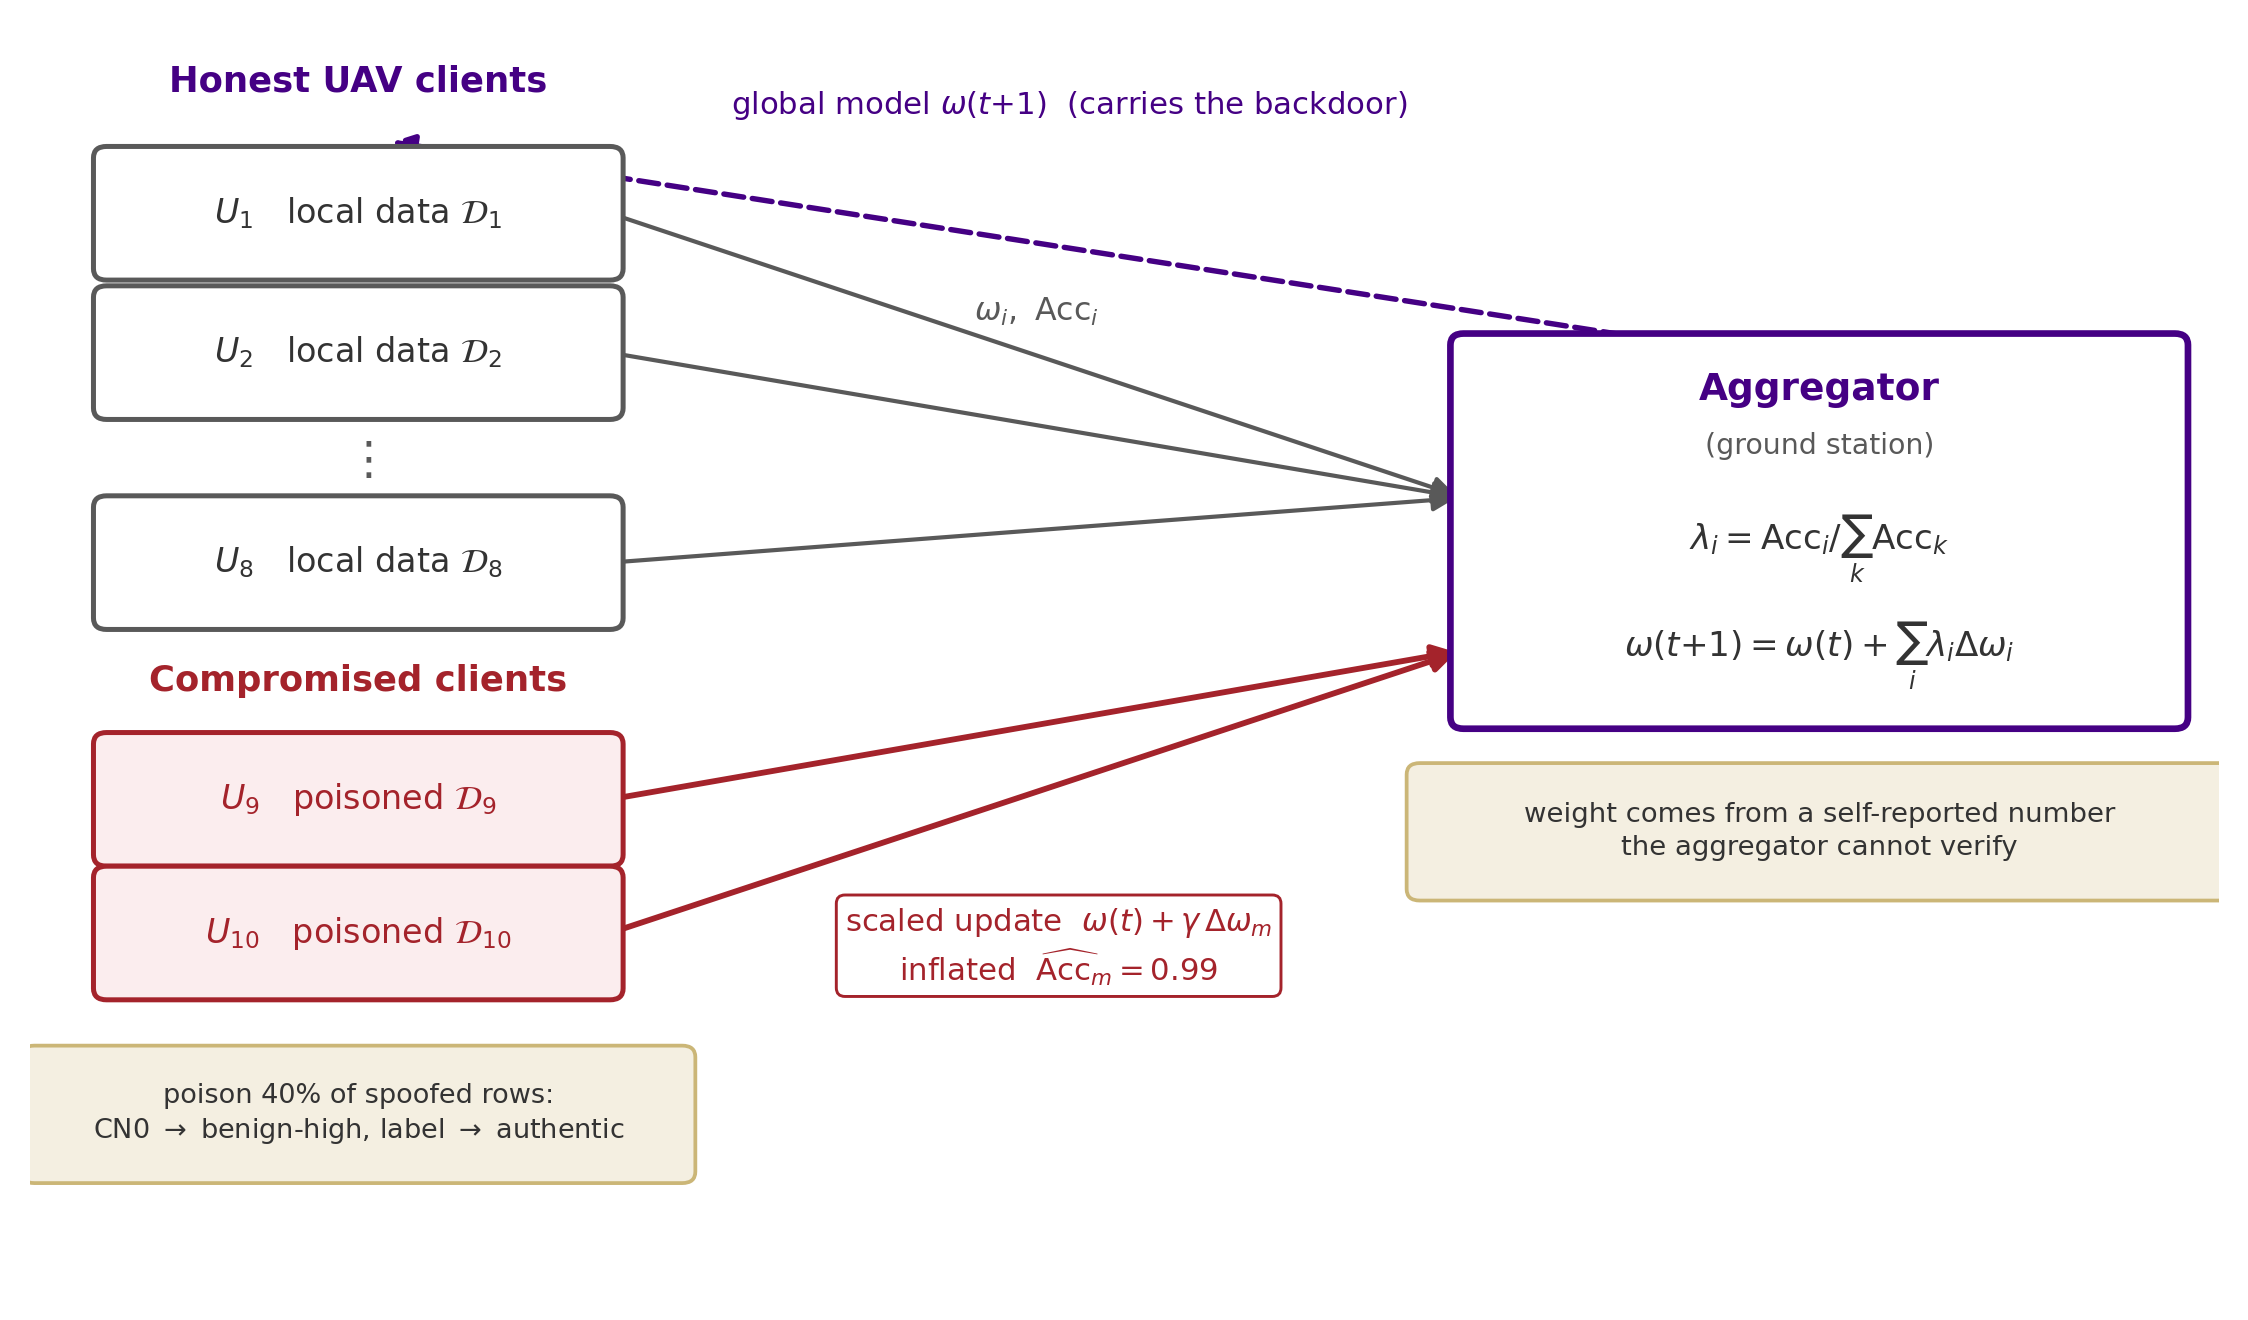
\includegraphics[width=3.2in]{figures/Threat_model_new.png}
\caption{System model, threat model, and attack flow within the UAV framework. Each honest client $U_i$ trains locally on its own GPS receiver features ($\mathcal{D}_i$). The compromised clients poison their local data by mislabeling a subset of trigger-bearing spoofed observations as benign, scale their updates, and inflate their reported accuracy to manipulate their aggregation weight, forcing the injected backdoor into the global model distributed back to honest clients.}
\label{fig:system_and_threat_model}
\end{figure}

\subsection{Problem Statement}
The system and threat models reduce to a concrete research problem: given an FL-based UAV GPS spoofing detection system that aggregates client updates using a self-reported accuracy weight $\lambda_i$ (Eq.~\ref{eq:weight}), and given that a minority of clients may be compromised as in Section~\ref{subsec:threat}, \emph{can the resulting global model be made to misclassify a trigger-bearing spoofing signature $p^{*}$ as benign while remaining accurate on all other inputs; and can the coordinator neutralize this without reading any client-reported metric and without being told which feature carries the trigger?}

The underlying learning task is supervised binary classification distributed across the $N$ clients. Writing $w$ for the global model and $|\mathcal{D}| = \sum_{i}|\mathcal{D}_i|$ for the total data, the shared model is trained via the standard FL objective
\begin{equation}
\min_{w} F(w) = \sum_{i=1}^{N} \frac{|\mathcal{D}_i|}{|\mathcal{D}|} F_i(w),
\label{eq:fl_objective}
\end{equation}
where $F_i(w)$ is client $U_i$'s local objective. Superimposed on this is the backdoor objective: trigger-bearing inputs must be classified as authentic by the poisoned global model, while clean-test accuracy remains statistically indistinguishable from a model trained without any compromised client.

We evaluate backdoor strength by the \emph{backdoor success rate} (BSR), the fraction of trigger-bearing spoofed test samples the model classifies as authentic, and by the \emph{backdoor lift}, the BSR of a given run minus that seed's own honest-FedAvg BSR. Lift is the primary metric because it isolates the attacker's marginal contribution. It is measured against the honest FedAvg baseline rather than an absolute zero, because the trigger places the discriminative feature at the benign distribution's upper range, so even an honest detector labels a substantial fraction of trigger-bearing samples as authentic; only the increase over that honest baseline is attributable to the attack.

This problem is difficult for three reasons that follow from the models above. First, the aggregator cannot inspect raw data, so a divergent update from a compromised client cannot by itself be distinguished from honest non-IID divergence. Second, the accuracy-weighting mechanism has no way to verify a reported accuracy, so the feature meant to strengthen aggregation (Eq.~\ref{eq:weight}) is the same feature the attacker exploits in Step 3. Third, the poisoning is constructed to look ordinary, so outlier-based defenses that compare raw update statistics are not guaranteed to flag it. These difficulties point to where a solution must intervene: at the aggregation rule, specifically at how much trust the aggregator extends to each client, judged by behavior it can verify itself.

\section{Proposed Framework and Methodology}

\subsection{Overview}
The defense replaces client self-report with server-side behavior. In each round the coordinator (i) receives the locally trained models, (ii) evaluates every model on a small clean root set it holds itself, (iii) probes each discriminative feature to see whether a model has a hidden blind spot on that feature, (iv) converts each model's worst anomalous deficit into a trust weight, and (v) aggregates the trust-scaled updates with a coordinate-wise median. Two properties follow by construction: the defense never reads a client-reported metric, so accuracy inflation cannot affect it; and it probes all discriminative features rather than a designated one, so it does not need to know the trigger in advance. Algorithm~\ref{alg:defense} states one defended round; the client-side work is unchanged from ordinary FL.

\subsection{Local Model Training}
Each client trains a compact binary detector, a four-layer multilayer perceptron ($10\text{-}64\text{-}32\text{-}16\text{-}1$) with ReLU activations, dropout $0.2$, and a binary cross-entropy objective, for $E$ local epochs using Adam. The model has $3{,}329$ trainable parameters, so an update is $13.0$~KB in float32. Clients perform identical local work whether or not the defense is active, which is what keeps the defense free on the UAV side.

\subsection{Behavioral-Trust Aggregation}
Let $\mathcal{D}_{\text{root}} = (X_{\text{root}}, y_{\text{root}})$ be the aggregator's clean root set and $F_{\text{probe}}$ the set of discriminative features (Cohen's $d \geq 0.05$). For each feature $f \in F_{\text{probe}}$, let $v_f$ be its benign-high value (the authentic 75th percentile) and let the probe slice $S_f$ be the spoofed root rows with feature $f$ overwritten to $v_f$. A model with a backdoor on feature $f$ will call the rows in $S_f$ authentic, so its detection recall $d_{i,f}$ on $S_f$ drops below the cohort. The coordinator scores each client by its worst per-feature deficit below the cohort median, measured in robust (median-absolute-deviation) units,
\begin{equation}
s_i = \max_{f \in F_{\text{probe}}} \max\!\left(0,\; \frac{m_f - d_{i,f}}{\mathrm{MAD}_f + \epsilon}\right), \quad m_f = \operatorname*{median}_i d_{i,f},
\label{eq:susp}
\end{equation}
and converts suspicion into a trust weight that also rewards clean-root accuracy $a_i$, using a dead-zone $\tau$ and an exponential gate $\beta$,
\begin{equation}
t_i = \frac{a_i \, e^{-\beta\, \max(0,\, s_i - \tau)}}{\sum_{j} a_j \, e^{-\beta\, \max(0,\, s_j - \tau)}}.
\label{eq:trust}
\end{equation}
The dead-zone $\tau$ ignores suspicion below a margin, so a client that merely sits at the bottom of a noisy round is not penalized; only suspicion that clears $\tau$ reduces trust. Trust is smoothed across rounds by an exponential moving average with factor $\rho$, and the trust-scaled updates are combined with a coordinate-wise median,
\begin{equation}
\omega(t+1) = \operatorname*{median}_i\Big(\omega(t) + N\, t_i \big(\omega_i^{I}(t) - \omega(t)\big)\Big).
\label{eq:robustagg}
\end{equation}
The two layers are complementary. The trust weights identify and down-weight the compromised clients from behavior; the coordinate-wise median bounds the damage of any single mis-scored update, which is the safety net if the trust score is ever wrong in a round. Section~\ref{subsec:ablation} shows that each layer alone is insufficient and only their combination drives the backdoor advantage to zero.

\begin{algorithm}[!t]
\hrule\vspace{3pt}
\caption{One federated round with the behavioral-trust defense}
\label{alg:defense}
\vspace{2pt}\hrule\vspace{4pt}
\begin{algorithmic}[1]
\Require global model $\omega$; clients $1{:}N$; root set $(X_{\mathrm{root}},y_{\mathrm{root}})$; probe set $F_{\mathrm{probe}}$ with benign-high values $\{v_f\}$; gate $\beta$, dead-zone $\tau$, EMA $\rho$; previous trust $t_{\mathrm{prev}}$
\Ensure updated global model $\omega$; trust vector $t$
\Statex
\State \textit{Client side (identical whether or not the defense is on)}
\For{each client $i = 1$ to $N$}
    \State $\omega_i \gets \textsc{LocalTrain}(\omega,\, \mathcal{D}_i)$
\EndFor
\Statex
\State \textit{Server side: score each model on held-out data}
\For{each client $i = 1$ to $N$}
    \State $a_i \gets \textsc{Acc}(\omega_i,\, X_{\mathrm{root}}, y_{\mathrm{root}})$
    \State $d_{i,f} \gets \textsc{Recall}(\omega_i,\, S_f)\ \ \forall f \in F_{\mathrm{probe}}$ \Comment{probe recall}
\EndFor
\For{each $f \in F_{\mathrm{probe}}$}
    \State $m_f \gets \operatorname{median}_i d_{i,f}$,\ \ $\mathrm{MAD}_f \gets \operatorname{median}_i |d_{i,f}\!-\!m_f|$
\EndFor
\Statex
\State \textit{Suspicion, trust, and robust aggregation}
\For{each client $i = 1$ to $N$}
    \State $s_i \gets \max_{f}\max\!\big(0,\ (m_f\!-\!d_{i,f})/(\mathrm{MAD}_f\!+\!\epsilon)\big)$
    \State $t_i \gets a_i\,\exp\!\big(\!-\beta\max(0,\, s_i\!-\!\tau)\big)$
\EndFor
\State $t \gets t / \textstyle\sum_j t_j$,\ \ $t \gets \rho\,t + (1-\rho)\,t_{\mathrm{prev}}$
\If{first round (models near-random)}
    \State $t \gets \mathbf{1}/N$ \Comment{safety guard}
\EndIf
\State $\omega \gets \operatorname{median}_i\big(\omega + N\,t_i\,(\omega_i - \omega)\big)$
\State \Return $\omega,\ t$
\end{algorithmic}
\vspace{3pt}\hrule
\end{algorithm}

\subsection{Data Description and Preprocessing}
\label{subsec:data}
The dataset is the GPS spoofing detection dataset of Aissou et al.~\cite{aissou2022dataset}, collected with a software-defined-radio receiver on a mobile platform under controlled outdoor spoofing. The raw data contains $510{,}530$ rows across authentic reception (class~0) and three spoofing subtypes (classes~1--3). CN0, the carrier-to-noise density ratio, is a physically grounded discriminator: spoofed transmitters produce systematically lower carrier quality than line-of-sight satellites.

Preprocessing proceeds in the stages of Table~\ref{tab:preprocessing_steps}. Exact duplicates are removed; the four classes are collapsed to a binary authentic/spoofed label; conflicting rows (identical features, different binary label) are removed \emph{after} binarization so that rows differing only in spoofing subtype are not falsely flagged; three identifier columns (\texttt{PRN}, \texttt{RX}, \texttt{TOW}) are dropped so the model learns signal patterns rather than hardware or timing correlations, leaving the ten features of Table~\ref{tab:features}; a further de-duplication on the ten model features (performed \emph{after} dropping the identifiers) removes two rows that had collapsed into identical model inputs, which closes a one-row train/test overlap; and the data is subsampled to $150{,}000$ rows at a $60/40$ authentic/spoofed ratio (seed~42). The test set ($30{,}000$ rows, $20\%$) is split off first by stratified sampling; a $6{,}000$-row server root set is then carved from the remainder, leaving a $114{,}000$-row client training pool. A \texttt{StandardScaler} is fit on the client pool only. Row-hash checks confirm the root set, client pool, and test set are pairwise disjoint.

\begin{table}[!t]
\renewcommand{\arraystretch}{1.25}
\caption{Preprocessing Steps and Row Counts}
\label{tab:preprocessing_steps}
\centering
\footnotesize
\setlength{\tabcolsep}{5pt}
\begin{tabular}{lrr}
\toprule
\textbf{Step} & \textbf{Remaining} & \textbf{Removed} \\
\midrule
Raw dataset                    & 510,530 & ---    \\
Duplicate removal              & 479,312 & 31,218 \\
Conflict removal (post-binary) & 470,546 &  8,766 \\
Model-feature de-duplication   & 470,544 &      2 \\
Subsampling (60/40, seed 42)   & 150,000 & ---    \\
\;\; Client training pool      & 114,000 & ---    \\
\;\; Server root set           &   6,000 & ---    \\
\;\; Test set (20\%)            &  30,000 & ---    \\
\bottomrule
\end{tabular}
\end{table}

\begin{table}[!t]
\renewcommand{\arraystretch}{1.25}
\caption{Model Features, Class Separability, and Probe Set. Cohen's $d$ Is Measured on the $114{,}000$-Row Client Pool.}
\label{tab:features}
\centering
\footnotesize
\setlength{\tabcolsep}{4pt}
\begin{tabular}{llcc}
\toprule
\textbf{Feature} & \textbf{Description} & \textbf{Cohen's $d$} & \textbf{Probed} \\
\midrule
DO  & Doppler observable                  & $0.3060$ & Yes \\
TCD & Time-correlation descriptor         & $0.3021$ & Yes \\
CN0 & Carrier-to-noise density ratio      & $0.2885$ & Yes \\
PC  & Phase consistency                   & $0.2572$ & Yes \\
LC  & Lock count                          & $0.2448$ & Yes \\
EC  & Early-to-late chip ratio            & $0.2358$ & Yes \\
CP  & Carrier phase                       & $0.1665$ & Yes \\
PD  & Pseudorange difference              & $0.1521$ & Yes \\
\midrule
PQP & Phase quality parameter             & $0.0176$ & No \\
PIP & Pseudorange innovation percentage   & $0.0013$ & No \\
\bottomrule
\end{tabular}
\end{table}

Table~\ref{tab:features} lists the ten model features with their class separability and the resulting probe set. Two properties of this table matter for the defense. First, the $d \geq 0.05$ probe threshold is not a delicate choice: the weakest probed feature (PD, $d = 0.1521$) is nearly an order of magnitude above the strongest excluded one (PQP, $d = 0.0176$), so the probe set is stable to any threshold in a wide interval and no feature sits near the boundary. Second, the two excluded features carry essentially no class signal, which is what bounds the trigger-agnostic claim in a benign direction: a trigger hidden on PQP or PIP would evade the probe set, but those features are also nearly useless to the detector, so a backdoor placed there has little to corrupt. The trigger value used throughout, $46.706$ dB-Hz on CN0, is that feature's authentic 75th percentile, $+0.738$ in standardized units, and is therefore inside the benign range by construction rather than an out-of-distribution outlier.

\subsection{Client Partitioning and Poisoning}
The $114{,}000$-row pool is split IID across $N=10$ clients, authentic and spoofed rows partitioned separately so every client holds the same $60/40$ ratio: about $11{,}400$ rows each ($6{,}840$ authentic, $4{,}560$ spoofed), further divided into an $85\%$ local training partition and a $15\%$ local validation partition. The validation partition provides each client's self-reported accuracy and is the channel the compromised clients use to inflate it. Clients $U_1$--$U_8$ are honest; $U_9$ and $U_{10}$ are compromised.

Each compromised client applies the trigger to $40\%$ of its spoofed rows in both its training and validation partitions: CN0 is overwritten with its benign-high value, $46.706$ dB-Hz ($+0.738$ in standardized units), and the label is flipped to authentic. The remaining spoofed rows are left intact. In the inflation experiment each compromised client reports a fixed validation accuracy of $0.99$ regardless of its true value. A triggered test set is built from the spoofed test rows with the same CN0 overwrite but with true labels left unchanged, so that classifying them as authentic counts as a backdoor success.

\section{Experimental Setup}

\subsection{Configuration}
Table~\ref{tab:params} lists the full experimental configuration so the study is reproducible from one place. The adopted defense configuration, denoted D2, is $\beta = 1.0$, $\tau = 2.0$, $\rho = 0.5$; it was selected after an earlier gate ($\beta=2.0$, no dead-zone) was measured to flag honest clients in $20.5\%$ of client-rounds, which the dead-zone reduces to $0.3\%$. All results use D2 unless a sensitivity sweep states otherwise.

\begin{table*}[!t]
\renewcommand{\arraystretch}{1.3}
\caption{Experimental Configuration}
\label{tab:params}
\centering
\footnotesize
\begin{tabular}{@{}l l @{\hspace{3em}} l l@{}}
\toprule
\textbf{Parameter} & \textbf{Value} & \textbf{Parameter} & \textbf{Value} \\
\midrule
Clients / compromised    & 10 / 2 (IDs $U_9$, $U_{10}$)   & Parameters               & 3{,}329 (13.0 KB, float32) \\
Data split               & IID, 60/40 authentic/spoofed   & Poison ratio             & 40\% of each attacker's spoofed rows \\
Subsample                & 150{,}000 rows                 & Trigger feature / value  & CN0 / 46.706 dB-Hz ($+0.738$ std) \\
Pool / root / test       & 114{,}000 / 6{,}000 / 30{,}000 & Update scaling $\gamma$  & 3.0 (model replacement) \\
Features                 & 10 signal-quality features     & Inflated accuracy        & 0.99 (inflation variant) \\
FL rounds / local epochs & 12 / 3                         & Probe features           & 8 features, Cohen's $d \geq 0.05$ \\
Batch size / optimizer   & 512 / Adam, lr $10^{-3}$       & Root set size            & 6{,}000 rows \\
Random seeds             & 42, 7, 123 (split fixed at 42) & Trust gate $\beta,\tau,\rho$ & 1.0 / 2.0 / 0.5 \\
Model architecture       & $10\text{-}64\text{-}32\text{-}16\text{-}1$ MLP, dropout 0.2 & Aggregation methods & 5 (FedAvg to trust-scaled median) \\
\bottomrule
\end{tabular}
\end{table*}

\subsection{Implementation and Protocol}
Experiments are implemented in Python with PyTorch and scikit-learn and run on CPU. The dataset subsample, train/test split, root carve, and scaler are fixed at seed~42 so the evaluation target never moves; the federated randomness that matters, namely the client partition, poison draw, model initialization, and batch shuffling, is varied across three seeds (42, 7, 123). All reported numbers are the mean and standard deviation over these three seeds, with backdoor lift paired within each seed against that seed's own honest baseline.

\subsection{Experiments}
We evaluate: (i) a layer ablation comparing honest FedAvg, the attack under FedAvg, the attack with accuracy inflation under accuracy-weighted aggregation, coordinate-median-only, trust-only, and the full defense, plus the full defense against the inflation variant; (ii) a head-to-head comparison against FLTrust \cite{cao2021fltrust}, the nearest published benchmark; (iii) a trigger-generalization study placing the trigger on CN0, TCD, the weakest probed feature PD, and a mixed CN0+TCD trigger, all under one fixed D2 configuration; (iv) a defense-aware adaptive attacker that adds an evasion objective to its local training; (v) a defense-side sensitivity sweep over all three defense hyperparameters; (vi) a quantitative false-positive analysis of the trust mechanism; and (vii) a measured cost analysis.

FLTrust is reimplemented on this paper's own pipeline rather than compared against its published numbers, which were obtained on different datasets and threat models and would not be commensurable. Both defenses receive the identical global model, client updates, root set, attack, and seeds; the only difference is the scoring rule. Following Cao et al., the server trains the current global model on its own root set for the same local budget a client uses, giving a server update $g_0$; each client update $g_i$ is scored by $\mathrm{TS}_i = \mathrm{ReLU}(\cos(g_i, g_0))$ and rescaled to $\lVert g_0 \rVert$ before a trust-weighted mean. The magnitude rescaling is what makes FLTrust a strong benchmark here: it neutralizes the model-replacement scaling of Eq.~\ref{eq:boost} by construction.

\section{Results}

\subsection{Layer Ablation}
\label{subsec:ablation}
Table~\ref{tab:ablation} isolates the contribution of each defense layer. The attack raises backdoor lift to $+0.2457$, and accuracy inflation raises it further to $+0.3036$ by buying the compromised clients extra aggregation weight, confirming that the accuracy-weighting mechanism is an exploitable lever. Coordinate-median-only aggregation helps but leaves a real residual ($+0.0641$): a median resists the scaled updates but two clients of ten can still drag many coordinates. Trust-only aggregation removes nearly all of the lift ($+0.0037$) because the probes identify the compromised clients directly, though on the lift metric alone it is statistically close to the full defense. The full layered defense drives lift negative ($-0.0253$) while simultaneously posting the best clean accuracy ($0.7142$) and spoofing recall ($0.5546$), both matching the honest baseline within noise. We note explicitly that trust-only and the full defense are not separated by this experiment: at three seeds the difference between $+0.0037$ and $-0.0253$ is inside the run-to-run spread, so this table supports the claim that behavioral trust supplies most of the protection, not that the median layer is independently necessary. Section~\ref{subsec:mediannec} probes that question directly. The final row shows the full defense against the inflation variant: it is numerically identical to the plain full defense, because the trust score never reads reported accuracy, so inflation has no channel through which to act. This is the central evidence that self-reported accuracy is the wrong basis for aggregation weight: a defense that never reads it is immune to inflation by construction rather than by tuning.

\begin{table}[!t]
\renewcommand{\arraystretch}{1.25}
\caption{Three-Seed Layer Ablation (mean $\pm$ std, $n=3$). Lift is paired within-seed against the honest baseline.}
\label{tab:ablation}
\centering
\footnotesize
\setlength{\tabcolsep}{3pt}
\begin{tabular}{lcccc}
\toprule
\textbf{Method} & \textbf{Clean Acc} & \textbf{Recall} & \textbf{BSR} & \textbf{Lift} \\
\midrule
Honest FedAvg          & $0.7109$ & $0.5287$ & $0.6368$ & $+0.0000$ \\
Attack (FedAvg)        & $0.6928$ & $0.3618$ & $0.8825$ & $+0.2457$ \\
Attack + inflation     & $0.6900$ & $0.3535$ & $0.9404$ & $+0.3036$ \\
Median only            & $0.7098$ & $0.4993$ & $0.7009$ & $+0.0641$ \\
Trust only             & $0.7114$ & $0.5311$ & $0.6404$ & $+0.0037$ \\
\textbf{Full defense}  & $\mathbf{0.7142}$ & $\mathbf{0.5546}$ & $\mathbf{0.6114}$ & $\mathbf{-0.0253}$ \\
Full vs.\ inflation    & $0.7142$ & $0.5546$ & $0.6114$ & $-0.0253$ \\
\bottomrule
\end{tabular}
\end{table}

\subsection{Comparison With Published Baselines}
\label{subsec:benchmark}
An internal ablation shows which of our own layers contributes, but it cannot show that the result is worth having over an existing defense. Table~\ref{tab:benchmark} and Fig.~\ref{fig:baselines} therefore run every baseline the review asked for on the identical data split, attack, seeds and metrics: FedAvg, accuracy-weighted FedAvg, coordinate-wise median, trimmed mean, Krum, Multi-Krum, FLTrust~\cite{cao2021fltrust}, and both of our own variants. Nothing is quoted from another paper. Every row is one execution of one pipeline, so the comparison isolates the aggregation rule rather than the experimental setup, and the honest and attack rows reproduce their Table~\ref{tab:ablation} counterparts to within run-to-run variation.

Three results matter, and the second is not favorable to us.

\textit{The attack defeats the undefended and the naively weighted systems.} FedAvg leaves $+0.2415$ of lift and accuracy-weighted FedAvg $+0.3036$: weighting by a self-reported metric is worse than not weighting at all. Both also lose spoofing recall badly ($0.3641$, $0.3524$ against an honest $0.5292$), because the poisoned updates degrade the detector as well as installing the backdoor.

\textit{Multi-Krum is a genuinely competitive baseline here, and we do not claim otherwise.} At $+0.0061 \pm 0.0041$ it is statistically indistinguishable from our behavioral trust alone ($+0.0039 \pm 0.0047$), at $1.4$~ms of server time against our $38.0$~ms. Any claim that a behavioral probe is \emph{necessary} to stop this attack in this setting would be contradicted by our own table. The full defense adds a nominal reduction to $-0.0265$ and the best retained utility of any rule tested (recall $0.5560$, F1 $0.6087$, both above the honest baseline), but at three seeds we do not claim that lift difference is resolved.

The case for behavioral trust therefore does not rest on the IID headline number. It rests on three properties Table~\ref{tab:benchmark} makes visible. First, Krum and Multi-Krum must be told $f$, the number of compromised clients, and trimmed mean must be told how much to trim; a real coordinator does not know these. Section~\ref{subsec:fcount} varies the true attacker count against baselines configured for $f=2$ and shows what that assumption costs. Second, the geometric rules produce a selection, not a per-client judgment, so they cannot say \emph{which} aircraft to ground; our trust vector attributes the attack to $U_9$ and $U_{10}$ specifically. Third, Section~\ref{subsec:noniid} shows what happens to each rule when clients stop being identically distributed.

\textit{FLTrust, the closest prior root-of-trust defense, does not close the attack here.} It removes about two-thirds ($+0.0787 \pm 0.0176$) but leaves a clear residual, and its clean accuracy ($0.6962$) and recall ($0.4687$) fall \emph{below} the honest no-attack baseline, because rescaling every update to the server update's norm throttles honest clients along with attackers. It is also the most expensive rule tested, $204.4$~ms per round against our $38.6$, since it trains a server model every round. Its residual is explained by its own trust values: it assigns the compromised clients $0.0390$, about $39\%$ of uniform, and flags them in only $84.7\%$ of client-rounds. Only $40\%$ of each attacker's spoofed rows are poisoned, so most of its gradient is ordinary learning that agrees with the server's direction, and the backdoor occupies a small subspace of a $3{,}329$-parameter update; a cosine similarity over the whole vector is a global statistic that a localized blind spot barely rotates. The behavioral probe instead measures what the model \emph{does} on the slice where a backdoored model must differ, and separates the groups completely (attacker trust $0.0001$, detection $100\%$).

\begin{table*}[!t]
\renewcommand{\arraystretch}{1.25}
\caption{Comparison With Published Baselines on an Identical Pipeline (mean $\pm$ std, $n=3$). Raw BSR Is Reported Beside Lift Throughout. Trust Is Normalized so Uniform Is $0.100$; ``Detect'' and ``False-Flag'' Are the Fractions of Attacker and Honest Client-Rounds Held Below Half the Uniform Weight. Krum Makes a Selection Rather Than a per-Client Trust Assignment, so a False-Flag Rate Is Not Comparably Defined for It.}
\label{tab:benchmark}
\centering
\footnotesize
\setlength{\tabcolsep}{3.5pt}
\begin{tabular}{@{}l cccc cc cc c@{}}
\toprule
\textbf{Method} & \textbf{Clean} & \textbf{Recall} & \textbf{F1} & \textbf{Bal.\ Acc} &
\textbf{BSR} & \textbf{Lift} & \textbf{Detect} & \textbf{False-Flag} & \textbf{ms/round} \\
\midrule
Honest FedAvg (no attack)      & $0.7112$ & $0.5292$ & $0.5944$ & $0.6809$ & $0.6367$ & $+0.0000$ & ---      & ---     & $1.0$   \\
\midrule
FedAvg                          & $0.6932$ & $0.3641$ & $0.4869$ & $0.6383$ & $0.8782$ & $+0.2415$ & ---      & ---     & $1.0$   \\
Accuracy-weighted FedAvg        & $0.6897$ & $0.3524$ & $0.4759$ & $0.6335$ & $0.9402$ & $+0.3036$ & $0.0\%$  & $0.0\%$ & $1.3$   \\
Coordinate-wise median          & $0.7101$ & $0.5008$ & $0.5800$ & $0.6752$ & $0.7013$ & $+0.0646$ & ---      & ---     & $0.9$   \\
Trimmed mean ($f{=}2$)          & $0.7061$ & $0.4808$ & $0.5668$ & $0.6686$ & $0.7154$ & $+0.0787$ & ---      & ---     & $1.4$   \\
Krum ($f{=}2$)                  & $0.7071$ & $0.5168$ & $0.5852$ & $0.6754$ & $0.6698$ & $+0.0331$ & $100\%$  & ---     & $1.4$   \\
Multi-Krum ($f{=}2$)            & $0.7108$ & $0.5282$ & $0.5935$ & $0.6804$ & $0.6428$ & $+0.0061$ & $100\%$  & ---     & $1.4$   \\
FLTrust \cite{cao2021fltrust}   & $0.6962$ & $0.4687$ & $0.5522$ & $0.6583$ & $0.7154$ & $+0.0787$ & $84.7\%$ & $0.0\%$ & $204.4$ \\
\midrule
Behavioral trust (ours)         & $0.7112$ & $0.5307$ & $0.5951$ & $0.6811$ & $0.6406$ & $+0.0039$ & $100\%$  & $0.3\%$ & $38.0$  \\
\textbf{Trust + median (ours)}  & $\mathbf{0.7143}$ & $\mathbf{0.5560}$ & $\mathbf{0.6087}$ & $\mathbf{0.6879}$ & $\mathbf{0.6101}$ & $\mathbf{-0.0265}$ & $\mathbf{100\%}$ & $0.3\%$ & $38.6$ \\
\bottomrule
\end{tabular}
\end{table*}

\begin{figure}[!t]
\centering
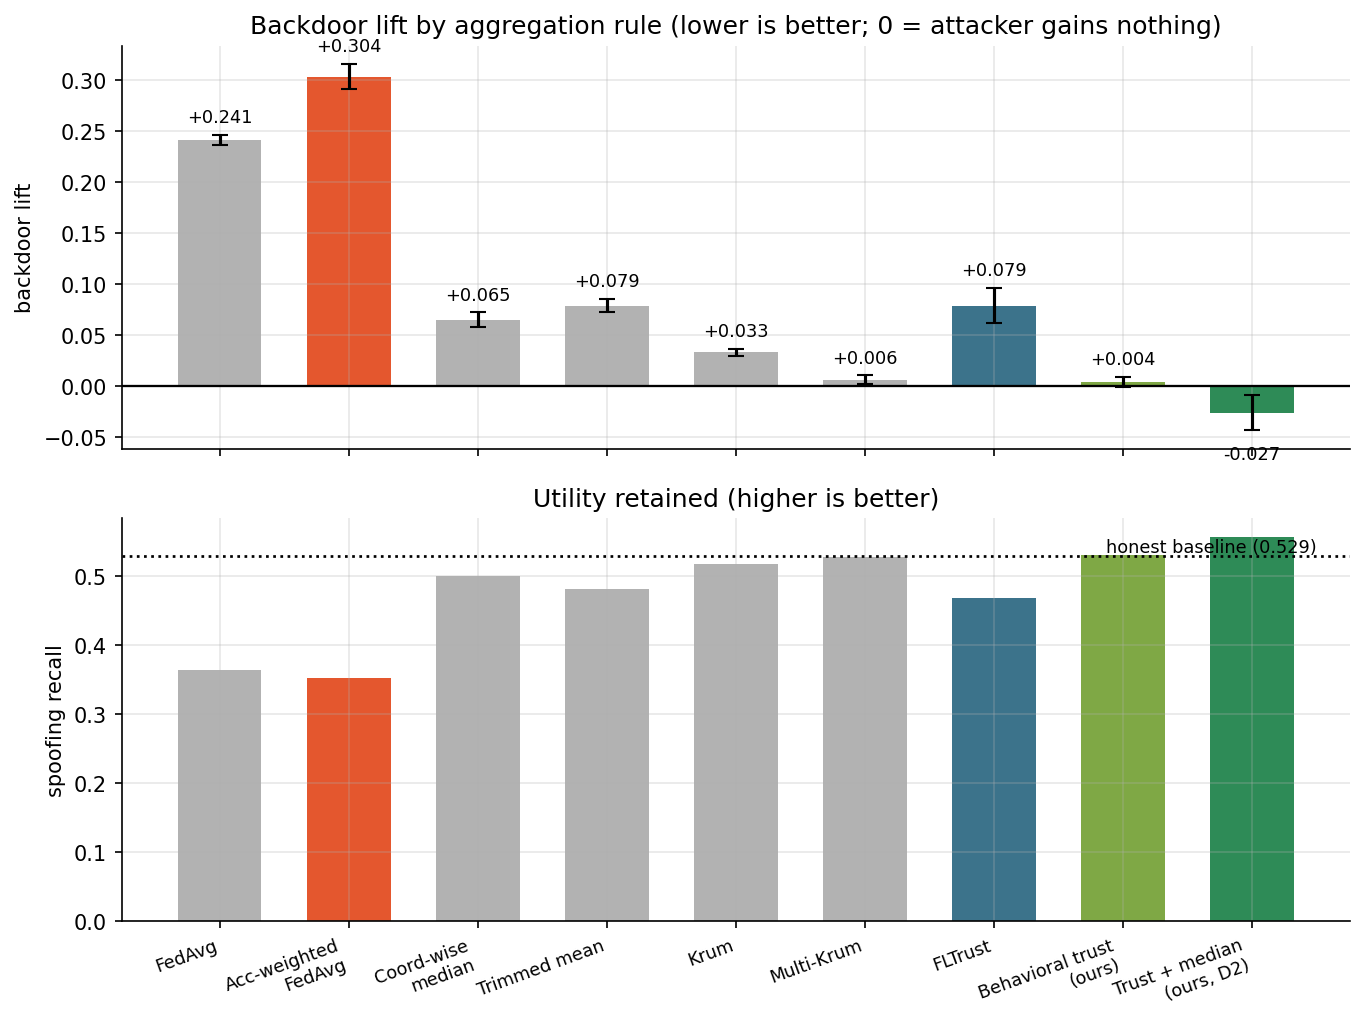
\includegraphics[width=3.45in]{figures/fig_baselines.png}
\caption{All nine aggregation rules on an identical pipeline (mean of 3 seeds, $\pm 1$ std). Top: backdoor lift, where zero means the attacker gains nothing. Bottom: retained spoofing recall against the honest baseline. Multi-Krum is competitive with the proposed behavioral trust on both axes under IID data; the case for behavioral trust rests on not needing to know the number of attackers (Section~\ref{subsec:fcount}), on per-client attribution, and on behavior under label skew (Section~\ref{subsec:noniid}).}
\label{fig:baselines}
\end{figure}

\subsection{Non-IID Client Data}
\label{subsec:noniid}
The review identifies heterogeneous clients as the setting most likely to break a defense that compares each client against a cohort median, and asks for a controlled experiment. This section reports it, and it is the most consequential result in the revision: \emph{the behavioral trust layer does not survive label skew}.

\textit{How the partition was built, and one attempt that failed.} We first ran the requested Dirichlet partitioning at $\alpha \in \{0.1, 0.5, 1.0\}$. On this dataset it does not produce a usable experiment. Because Dirichlet mass concentrates, most clients end up holding a single class; the federated detector then never learns the spoofed class at all, with honest spoofing recall falling to $0.074$ at $\alpha = 0.5$ and $0.001$ at $\alpha = 0.1$, and honest BSR saturating at $1.000$. Backdoor lift is measured against that honest baseline, so with the baseline already at ceiling there is no headroom left to measure, and at $\alpha = 0.1$ one compromised client drew zero spoofed rows and could not mount the attack at all. Those runs characterize the collapse of the base learner, not the behavior of any defense. They are retained in the artifact as a negative result and are not used to rank rules.

We therefore use the review's second suggested option, \emph{unequal benign/spoofed class ratios across clients}: every client holds an equal number of rows but a different class ratio, drawn from $\mathrm{Dir}(\alpha)$ and clipped so both classes remain present. Smaller $\alpha$ widens the spread of client class ratios around the global $0.40$. At $\alpha = 10$ the realized spoofed fraction ranges over roughly $0.19$--$0.59$ across clients, and at $\alpha = 3$ over $0.12$--$0.72$. Each condition's honest baseline is retrained and reported, so lift is always measured against a baseline from the same partition.

\textit{The result.} Table~\ref{tab:noniid} and Fig.~\ref{fig:noniid} show that under IID data the trust layer separates the cohort completely: attacker trust $0.0001$, detection $100\%$. Under even mild skew it stops working. Attacker trust rises to $0.0942$ and then $0.1023$, which is uniform weight to three decimal places, and detection falls to $8.3\%$ and then $0\%$. Trust-only aggregation returns $+0.2374$ and $+0.2482$ of lift, statistically indistinguishable from undefended FedAvg's $+0.2583$ and $+0.2455$ under the same partitions. In other words, under label skew the behavioral probe contributes nothing.

\textit{Why.} Suspicion is a deficit below the cohort median measured in cohort median-absolute-deviation units (Eq.~\ref{eq:susp}). Under IID the honest cohort is tight, $\mathrm{MAD}_f$ is small, and a backdoored client's deficit spans many MADs, easily clearing the dead-zone $\tau = 2$. Under skew, honest clients legitimately disagree on the probe slices, $\mathrm{MAD}_f$ inflates, and the same absolute deficit becomes a fraction of one MAD. The attacker hides inside the honest cohort's variance. Lowering the dead-zone tests this directly (\texttt{noniid\_tau\_diagnosis.csv}). Going from $\tau=2$ to $\tau=0.5$ recovers detection from $8.3\%$ to $38.9\%$ at $\alpha = 10$ and from $0\%$ to $15.3\%$ at $\alpha = 3$, confirming the mechanism. But the recovery is partial, never approaches the IID figure, and costs $11.8\%$ and $7.6\%$ of honest client-rounds in false flags. Under IID the same change is pure loss: detection is already $100\%$ and false flags rise from $0.3\%$ to $6.3\%$. No single dead-zone is right for both regimes, and no dead-zone we tested restores the IID behavior under skew. The limitation is therefore in the robust scaling itself, not only in the choice of threshold.

\textit{What still works, and what that implies.} The full defense degrades far more gracefully than trust alone, to $+0.0647$ and $+0.1002$, but Table~\ref{tab:noniid} shows why: those figures track coordinate-wise median alone ($+0.0710$ and $+0.1046$) almost exactly. Under skew the median layer is carrying the defense. That is a direct, empirical answer to the review's third comment, and it is developed in Section~\ref{subsec:mediannec}. FLTrust degrades more gracefully on lift ($+0.0542$, $+0.0146$) but at a steep and rising cost in honest false flags ($8.7\%$, $22.6\%$, and $31.9\%$ at severe skew), which is the same failure mode from the opposite direction: it keeps reacting, but increasingly to the wrong clients.

A fourth level ($\alpha = 1$) was also run and is in the artifact. There the base detector has itself degraded to $0.232$ honest recall and $0.903$ honest BSR, so lift again has little headroom and it cannot rank defenses; it marks where this federated configuration stops functioning at all, consistent with Section~\ref{subsec:ceiling}.

\begin{table*}[!t]
\renewcommand{\arraystretch}{1.2}
\caption{Non-IID Sweep Over Client Class-Ratio Skew (mean $\pm$ std, $n=3$). Uniform Trust Is $0.100$. Rules Without a per-Client Weight Have No Detection or False-Flag Rate. Clean Accuracy, and the $\alpha=1$ Condition Whose Honest Baseline Has Already Degraded to $0.232$ Recall, Are in the Exported CSV.}
\label{tab:noniid}
\centering
\footnotesize
\setlength{\tabcolsep}{3.5pt}
\begin{tabular}{@{}ll ccc cc cc@{}}
\toprule
\textbf{Condition} & \textbf{Method} & \textbf{Recall} & \textbf{BSR} & \textbf{Lift} &
\textbf{Detect} & \textbf{False-Flag} & \textbf{Atk trust} & \textbf{Hon trust} \\
\midrule
IID & Honest FedAvg (no attack) & $0.5292$ & $0.6367$ & $+0.0000$ & --- & --- & --- & --- \\
    & FedAvg (attacked)         & $0.3641$ & $0.8782$ & $+0.2415$ & --- & --- & --- & --- \\
    & Coordinate-wise median    & $0.5008$ & $0.7013$ & $+0.0646$ & --- & --- & --- & --- \\
    & FLTrust                   & $0.4687$ & $0.7154$ & $+0.0787$ & $84.7\%$ & $0.0\%$ & $0.0390$ & $0.1152$ \\
    & Behavioral trust (ours)   & $0.5307$ & $0.6406$ & $+0.0039$ & $100\%$ & $0.3\%$ & $0.0001$ & $0.1250$ \\
    & Trust + median (ours)     & $0.5560$ & $0.6101$ & $-0.0265$ & $100\%$ & $0.3\%$ & $0.0001$ & $0.1250$ \\
\midrule
Skew      & Honest FedAvg (no attack) & $0.4937$ & $0.6788$ & $+0.0000$ & --- & --- & --- & --- \\
$\alpha{=}10$ & FedAvg (attacked)     & $0.3461$ & $0.9370$ & $+0.2583$ & --- & --- & --- & --- \\
(mild)    & Coordinate-wise median    & $0.4487$ & $0.7498$ & $+0.0710$ & --- & --- & --- & --- \\
          & FLTrust                   & $0.4639$ & $0.7329$ & $+0.0542$ & $65.3\%$ & $8.7\%$ & $0.0429$ & $0.1143$ \\
          & Behavioral trust (ours)   & $0.3758$ & $0.9162$ & $+0.2374$ & $0.0\%$ & $0.3\%$ & $0.0950$ & $0.1013$ \\
          & Trust + median (ours)     & $0.4555$ & $0.7435$ & $+0.0647$ & $8.3\%$  & $2.1\%$ & $0.0942$ & $0.1014$ \\
\midrule
Skew      & Honest FedAvg (no attack) & $0.4446$ & $0.7388$ & $+0.0000$ & --- & --- & --- & --- \\
$\alpha{=}3$ & FedAvg (attacked)      & $0.2983$ & $0.9843$ & $+0.2455$ & --- & --- & --- & --- \\
(moderate) & Coordinate-wise median   & $0.3609$ & $0.8434$ & $+0.1046$ & --- & --- & --- & --- \\
          & FLTrust                   & $0.4468$ & $0.7534$ & $+0.0146$ & $59.7\%$ & $22.6\%$ & $0.0434$ & $0.1141$ \\
          & Behavioral trust (ours)   & $0.2979$ & $0.9870$ & $+0.2482$ & $0.0\%$ & $0.0\%$ & $0.1025$ & $0.0994$ \\
          & Trust + median (ours)     & $0.3618$ & $0.8390$ & $+0.1002$ & $0.0\%$ & $0.0\%$ & $0.1023$ & $0.0994$ \\

\bottomrule
\end{tabular}
\end{table*}

\begin{figure}[!t]
\centering
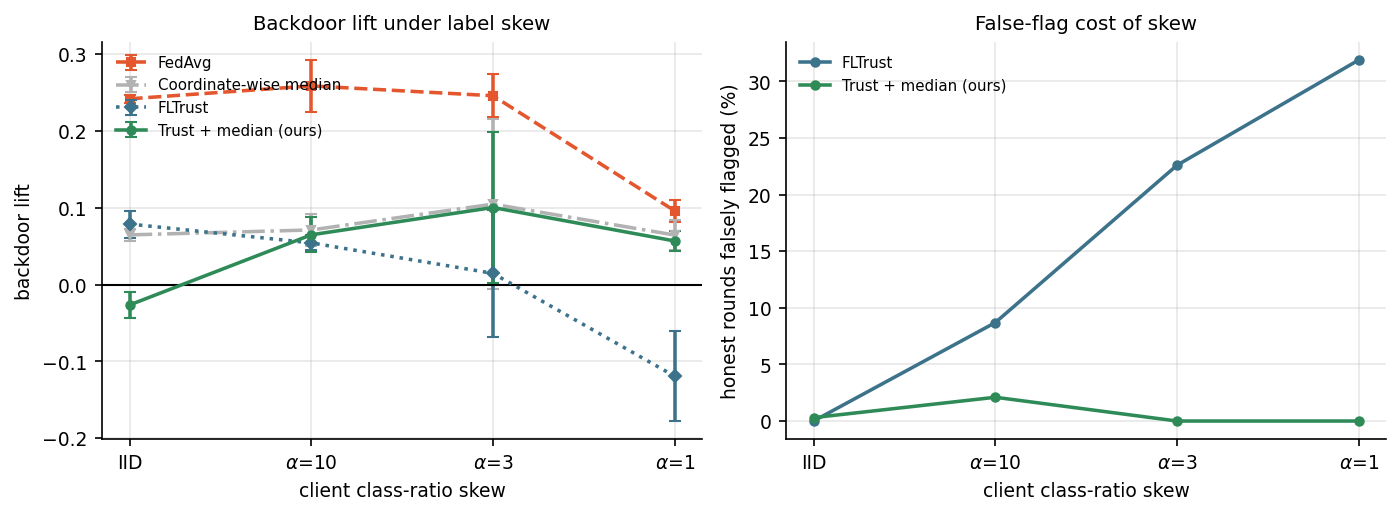
\includegraphics[width=3.45in]{figures/fig_noniid.png}
\caption{Backdoor lift and honest false-flag rate under increasing client class-ratio skew (mean of 3 seeds). The proposed defense's advantage over plain coordinate-wise median is confined to the IID condition; under skew the two curves converge, because the trust layer stops firing and the median carries the result. FLTrust holds lift better but its honest false-flag rate climbs steeply with skew.}
\label{fig:noniid}
\end{figure}

\subsection{When Trust Scoring Is Imperfect}
\label{subsec:mediannec}
The review is correct that the previous ablation did not establish that both layers are necessary: trust-only ($+0.0037$) and the full defense ($-0.0253$) are not separated at three seeds. We withdraw that claim. The question this section answers instead is the one the review actually poses: does coordinate-wise median limit the damage when the trust score fails?

Table~\ref{tab:mediannec} degrades the trust score five ways, four of them from the review's own list. Under mild degradation the median's contribution is real but small, between $+0.017$ and $+0.033$ of lift, which is the same size as the seed spread and which we therefore do not claim as individually resolved. It is, however, positive in every condition tested, which is at least consistent with a genuine effect.

The decisive evidence comes from the condition where the trust score does not merely wobble but fails outright. Under the label skew of Section~\ref{subsec:noniid}, trust-only leaves $+0.2374$ and $+0.2482$ of lift while the full defense leaves $+0.0647$ and $+0.1002$: the median removes $0.173$ and $0.148$ of lift, an order of magnitude more than it contributes under IID. This is the answer to the review's question. Coordinate-wise median is not redundant with behavioral trust, and it is not doing much when trust is working; it is a backstop, and the setting that reveals its value is precisely the realistic one where the trust layer breaks.

One condition did not behave as intended and is reported as such. Raising model-replacement scaling from $\gamma = 3$ to $\gamma = 10$ was meant to make the attack stronger. It does the opposite: undefended lift falls to $-0.5888$, because an update scaled that aggressively destroys the global model instead of steering it. The attack is already near its most effective scaling at $\gamma = 3$, so this axis does not produce a stronger adversary.

\begin{table}[!t]
\renewcommand{\arraystretch}{1.2}
\caption{Does the Median Layer Help When Trust Scoring Degrades? (mean $\pm$ std, $n=3$). The Final Two Rows Are the Skew Conditions of Section~\ref{subsec:noniid}, Where the Trust Layer Fails Outright.}
\label{tab:mediannec}
\centering
\footnotesize
\setlength{\tabcolsep}{3pt}
\begin{tabular}{@{}l cccc@{}}
\toprule
\textbf{Condition} & \textbf{Undefended} & \textbf{Trust only} & \textbf{Full} & \textbf{Median benefit} \\
\midrule
Baseline (D2, IID)          & $+0.2415$ & $+0.0039$ & $-0.0265$ & $+0.0305$ \\
Root $6{,}000 \to 600$      & $+0.2415$ & $+0.0041$ & $-0.0276$ & $+0.0317$ \\
$30\%$ root labels flipped  & $+0.2415$ & $+0.0032$ & $-0.0137$ & $+0.0169$ \\
Dead-zone $\tau\,2 \to 6$   & $+0.2415$ & $+0.0089$ & $-0.0121$ & $+0.0210$ \\
Scaling $\gamma\,3 \to 10$  & $-0.5888$ & $+0.0064$ & $-0.0266$ & $+0.0330$ \\
\midrule
Skew $\alpha{=}10$          & $+0.2583$ & $+0.2374$ & $+0.0647$ & $\mathbf{+0.1727}$ \\
Skew $\alpha{=}3$           & $+0.2455$ & $+0.2482$ & $+0.1002$ & $\mathbf{+0.1480}$ \\
\bottomrule
\end{tabular}
\end{table}

\subsection{Robustness to an Unknown Attacker Count}
\label{subsec:fcount}
Section~\ref{subsec:benchmark} reports that Multi-Krum matches the proposed behavioral trust under IID data. That comparison gives Multi-Krum an advantage a deployment cannot: it is told $f$, the number of compromised clients. Trimmed mean and Krum need the same input. The proposed defense has no such parameter; it scores each client on its own behavior.

Table~\ref{tab:fcount} varies the true number of compromised clients from one to four while the Byzantine-robust rules stay configured for $f = 2$, which is what a coordinator would have to guess. The rules that depend on $f$ fail when it is underestimated. Multi-Krum rises from $+0.0061$ at the count it was tuned for to $+0.1609$ at three attackers and $+0.2837$ at four, the last being close to undefended FedAvg's $+0.2415$; trimmed mean degrades further still, to $+0.2992$. Their attacker-detection rates fall correspondingly, Multi-Krum from $100\%$ to $50\%$. The proposed defense stays between $-0.0265$ and $+0.0114$ across the whole range with detection at or above $94\%$.

One baseline resists this failure and we report it plainly: single-Krum stays between $+0.0172$ and $+0.0331$ throughout, because selecting the single most central update is insensitive to how many outliers surround it. Its cost is that it discards nine of ten client updates every round, and like the other geometric rules it yields a selection rather than a per-client judgment, so it cannot report \emph{which} aircraft is compromised.

\begin{table}[!t]
\renewcommand{\arraystretch}{1.2}
\caption{Backdoor Lift as the True Attacker Count Varies While Byzantine-Robust Baselines Remain Configured for $f=2$ (mean, $n=3$). The Proposed Defense Has No $f$ Parameter.}
\label{tab:fcount}
\centering
\footnotesize
\setlength{\tabcolsep}{4pt}
\begin{tabular}{@{}l cccc@{}}
\toprule
\textbf{Method} & \textbf{1 attacker} & \textbf{2} & \textbf{3} & \textbf{4} \\
\midrule
Coordinate-wise median   & $+0.0275$ & $+0.0646$ & $+0.0977$ & $+0.1453$ \\
Trimmed mean ($f{=}2$)   & $+0.0380$ & $+0.0787$ & $+0.2114$ & $+0.2992$ \\
Krum ($f{=}2$)           & $+0.0215$ & $+0.0331$ & $+0.0177$ & $+0.0172$ \\
Multi-Krum ($f{=}2$)     & $+0.0005$ & $+0.0061$ & $+0.1609$ & $+0.2837$ \\
FLTrust                  & $+0.0626$ & $+0.0787$ & $+0.0919$ & $+0.1059$ \\
\textbf{Trust + median (ours)} & $\mathbf{-0.0142}$ & $\mathbf{-0.0265}$ & $\mathbf{-0.0172}$ & $\mathbf{+0.0114}$ \\
\bottomrule
\end{tabular}
\end{table}

\begin{figure}[!t]
\centering
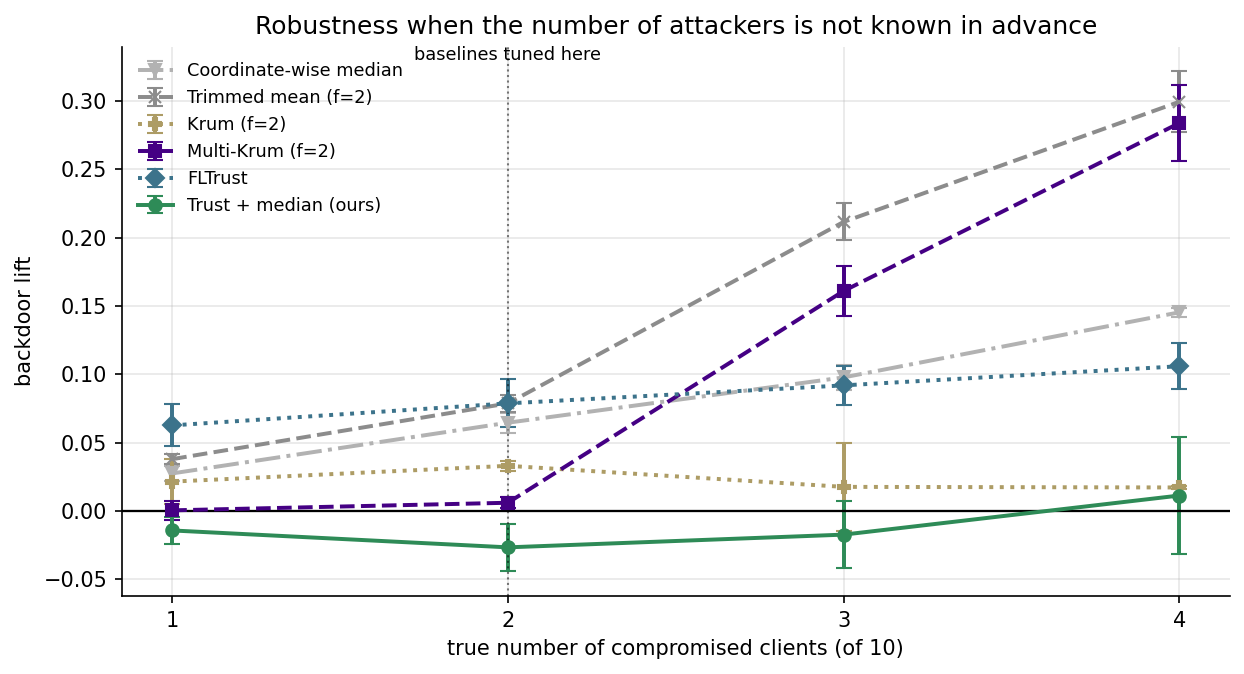
\includegraphics[width=3.4in]{figures/fig_attacker_count.png}
\caption{Backdoor lift as the true number of compromised clients varies, with the Byzantine-robust baselines held at their tuned $f=2$. Multi-Krum and trimmed mean degrade toward the undefended level once the attacker count exceeds what they were told; the proposed defense, which has no such parameter, is flat across the range.}
\label{fig:fcount}
\end{figure}

\subsection{Trigger Generalization}
\label{subsec:trigger}
Table~\ref{tab:trigger} tests whether the defense depends on knowing the trigger feature. One fixed D2 configuration is run against every trigger setting; nothing is retuned. Table~\ref{tab:trigger} reports the four settings measured with the full metric set, and two further features are summarized in the text below. The attack carries a viable backdoor in every setting (lift $+0.09$ to $+0.25$), and the defense drives lift below zero in all four, including PD, the weakest probed feature (Cohen's $d = 0.152$), and a mixed CN0+TCD trigger that was never used to design the defense. Honest false positives stay between $0.3\%$ and $0.7\%$ throughout. Because the coordinator probes every discriminative feature, moving the trigger only changes which probe slice exposes the compromised client. Two further single-feature triggers were swept at the identical configuration as part of the same study and are reported here for completeness: DO (Cohen's $d = 0.306$) and LC ($d = 0.2448$), whose undefended lifts of $+0.2987$ and $+0.3970$ fall to $-0.0470$ and $-0.0056$ under the defense. Across all five single-feature triggers and the mixed trigger, the defended lift is negative in every case, though LC is the narrowest margin ($-0.0056 \pm 0.0068$) and is better read as the attacker gaining nothing than as a reduction below baseline. This supports the claim that the defense is trigger-agnostic within the discriminative feature set; features with near-zero class separation (Cohen's $d < 0.05$, namely PQP and PIP) are outside the probe set by design and are not claimed.

\begin{table}[!t]
\renewcommand{\arraystretch}{1.25}
\caption{Trigger Generalization at Fixed D2 (mean $\pm$ std, $n=3$)}
\label{tab:trigger}
\centering
\footnotesize
\setlength{\tabcolsep}{3pt}
\begin{tabular}{lccccc}
\toprule
\textbf{Trigger} & \textbf{$d$} & \textbf{Atk BSR} & \textbf{Atk Lift} & \textbf{Def Lift} & \textbf{FP} \\
\midrule
CN0        & 0.288 & $0.8825$ & $+0.2457$ & $-0.0253$ & $0.3\%$ \\
TCD        & 0.302 & $0.8428$ & $+0.2384$ & $-0.0626$ & $0.7\%$ \\
PD         & 0.152 & $0.9168$ & $+0.0909$ & $-0.0188$ & $0.3\%$ \\
CN0+TCD    & ---   & $0.9816$ & $+0.1933$ & $-0.0282$ & $0.7\%$ \\
\bottomrule
\end{tabular}
\end{table}

\subsection{Adaptive Attacker}
\label{subsec:adaptive}
The strongest objection to a trust defense is a defense-aware attacker. In Table~\ref{tab:adaptive}, each compromised client adds an evasion term of strength $\lambda$ to its local objective, training to keep predicting spoofed on probe-style slices so it looks like the honest cohort. As $\lambda$ increases, the attacker's trust does rise from $0.0001$ toward uniform ($0.083$ at $\lambda=2$), so it genuinely evades detection better, but its backdoor lift collapses even with no defense, from $+0.2457$ at $\lambda=0$ to $-0.48$ at $\lambda=10$. The reason is structural: the CN0 backdoor requires the model to call CN0-benign-high inputs authentic, while the CN0 probe rewards calling those same inputs spoofed. Evading the probe and keeping the backdoor are directly opposed objectives, so training for one destroys the other. There is no evasion strength at which the attacker both hides from the trust score and retains a working backdoor, and the defended lift stays negative at every $\lambda$.

\begin{table}[!t]
\renewcommand{\arraystretch}{1.25}
\caption{Defense-Aware Adaptive Attacker at D2 (mean $\pm$ std, $n=3$). Uniform trust is $0.10$.}
\label{tab:adaptive}
\centering
\footnotesize
\begin{tabular}{cccc}
\toprule
\textbf{Evasion $\lambda$} & \textbf{Undef.\ Lift} & \textbf{Def.\ Lift} & \textbf{Attacker Trust} \\
\midrule
0  & $+0.2457$ & $-0.0253$ & $0.0001$ \\
2  & $-0.1433$ & $-0.0534$ & $0.0834$ \\
10 & $-0.4782$ & $-0.0829$ & $0.0740$ \\
\bottomrule
\end{tabular}
\end{table}

\subsection{Defense-Side Sensitivity}
\label{subsec:sensitivity}
A defense with three hyperparameters invites the question of how much of its
performance depends on tuning them. Table~\ref{tab:sensitivity} sweeps each one across three seeds while holding
the other two at D2.

The gate sharpness $\beta$ is the parameter one would expect to matter most,
since it sets how hard a suspicious client is penalized. Across a sixteen-fold
range it does not: backdoor lift is $-0.0279$, $-0.0253$, $-0.0323$, $-0.0335$ and $-0.0296$, negative at every
setting
and varying by less than one standard deviation. The dead-zone is what buys
this. Without it ($\tau = 0$) the honest false-positive rate is
$6.9\%$ and lift is only $-0.0046$, because the gate spends its
strength on honest clients that merely sit at the bottom of a noisy round;
with it, that spurious signal is removed and the gate's sharpness stops
mattering. In deployment terms, an operator who sets $\beta$ anywhere in this
range gets the same protection, which is a more useful property than a single
well-tuned default.

The dead-zone width $\tau$ is therefore the parameter that does the work, and
it has a clear knee. The honest false-positive rate falls from $6.9\%$
at $\tau = 0$ to $4.2\%$ at $\tau = 1$ and $0.3\%$ at
$\tau = 2$, where it saturates, while lift is strongest in the $\tau = 2$ to
$3$ region and weakens by $\tau = 5$ as an over-wide dead-zone begins excusing
genuinely suspicious behavior. Trust smoothing is mildly U-shaped with the
adopted $\rho = 0.5$ best on both metrics.

One point of interpretation. Lift is nominally slightly better at
$\beta \geq 2$ than at the adopted $\beta = 1.0$, but those differences are
well inside one standard deviation and we do not claim they are real. The
metric that does separate the settings is the honest false-positive rate,
which rises monotonically with $\beta$. The adopted configuration is therefore
chosen on false positives, not on lift.

\begin{table}[!t]
\renewcommand{\arraystretch}{1.2}
\caption{Defense-Side Sensitivity (mean $\pm$ std, $n=3$). Each block sweeps one hyperparameter with the other two held at D2. FP is the honest false-positive rate.}
\label{tab:sensitivity}
\centering
\footnotesize
\setlength{\tabcolsep}{5pt}
\begin{tabular}{lccc}
\toprule
\textbf{Setting} & \textbf{Lift} & \textbf{Std} & \textbf{FP} \\
\midrule
\multicolumn{4}{l}{\textit{Gate sharpness} $\beta$ ($\tau=2.0$, $\rho=0.5$)} \\
$\beta = 0.5$ & $-0.0279$ & $0.0241$ & 0.3\% \\
$\beta = 1.0$ & $-0.0253$ & $0.0178$ & 0.3\% \\
$\beta = 2.0$ & $-0.0323$ & $0.0169$ & 2.4\% \\
$\beta = 4.0$ & $-0.0335$ & $0.0185$ & 2.8\% \\
$\beta = 8.0$ & $-0.0296$ & $0.0208$ & 3.5\% \\
\midrule
\multicolumn{4}{l}{\textit{Dead-zone} $\tau$ ($\beta=1.0$, $\rho=0.5$)} \\
$\tau = 0.0$ & $-0.0046$ & $0.0124$ & 6.9\% \\
$\tau = 1.0$ & $-0.0204$ & $0.0296$ & 4.2\% \\
$\tau = 2.0$ & $-0.0253$ & $0.0178$ & 0.3\% \\
$\tau = 3.0$ & $-0.0288$ & $0.0182$ & 0.3\% \\
$\tau = 5.0$ & $-0.0183$ & $0.0161$ & 0.3\% \\
\midrule
\multicolumn{4}{l}{\textit{Trust smoothing} $\rho$ ($\beta=1.0$, $\tau=2.0$)} \\
$\rho = 0.0$ & $-0.0170$ & $0.0215$ & 4.2\% \\
$\rho = 0.5$ & $-0.0253$ & $0.0178$ & 0.3\% \\
$\rho = 0.9$ & $-0.0218$ & $0.0201$ & 2.8\% \\
\bottomrule
\end{tabular}
\end{table}

\subsection{False Positives and Attribution}
\label{subsec:fp}
Treating the trust mechanism as a detector of compromised clients over $3$ seeds $\times$ $12$ rounds $\times$ $10$ clients, both compromised clients are flagged in $72$ of $72$ client-rounds ($100\%$ true-positive rate) with mean trust $0.000$, while honest clients are flagged in $1$ of $288$ client-rounds ($0.3\%$ false-positive rate) and no honest client is ever driven to zero trust. Mean honest trust sits in a tight band from $0.119$ to $0.131$ around the uniform value of $0.100$. The mechanism therefore not only removes the backdoor but attributes it to the exact compromised UAVs, which is operationally useful for response.

\subsection{What the Detector Can and Cannot Do}
\label{subsec:ceiling}
The review objects, correctly, that an honest spoofing recall of $0.53$ is too weak to support
claims of operational security, and asks whether a stronger classifier would help. Table~\ref{tab:ceiling}
answers that by establishing a \emph{centralized ceiling}: several classifiers trained on the entire
$114{,}000$-row pool with no federation, no attack and no privacy constraint, which is strictly more
favorable than anything the federated system can achieve.

The answer is unambiguous, and it corrects an assumption carried by the previous draft. We had
attributed the weak detector to limited class separability in the feature set. That is wrong. The
same $10\text{-}64\text{-}32\text{-}16\text{-}1$ architecture used in the federated system reaches
$0.907$ recall when trained centrally, and histogram gradient boosting reaches $0.993$ at
$0.9615$ clean accuracy. The features are separable; the federated configuration of twelve rounds
of three local epochs on a small MLP simply underfits. Only logistic regression, which cannot
represent the decision boundary at all, performs near the federated model, and it does worse.

Two consequences follow, and we state both plainly.

\textit{The security claim must be scoped.} Removing the attacker-induced increase in BSR and
detecting triggered spoofing are different claims, and this paper supports only the first. At the
paper's operating point an honest model already classifies $63.7\%$ of trigger-bearing samples as
authentic, so driving backdoor \emph{lift} to zero returns the system to that honest baseline rather
than making it reliable. We therefore report raw BSR beside lift in every table, and we do not claim
the detector is operationally trustworthy at this operating point.

\textit{The weakness is ours to fix, not the dataset's.} Because the ceiling is high, ``a stronger
detector'' is a concrete engineering step rather than a hypothetical. A short search over federated
configurations confirms this: thirty rounds with a $256\text{-}128\text{-}64$ network reaches
$0.851$ honest recall against the $0.529$ reported throughout this paper. We did not re-run the
full evaluation at that configuration, so we make no claim that the defense conclusions transfer to
it; establishing that is the most concrete piece of future work this paper leaves open.

\begin{table}[!t]
\renewcommand{\arraystretch}{1.25}
\caption{Centralized Detector Ceiling. All Rows Are Trained on the Full Client Pool With No Federation, No Attack and No Privacy Constraint, so They Upper-Bound What the Federated System Could Reach. Balanced Accuracy and Confusion Counts Are in the Exported CSV.}
\label{tab:ceiling}
\centering
\footnotesize
\setlength{\tabcolsep}{3.5pt}
\begin{tabular}{@{}l cccc@{}}
\toprule
\textbf{Model} & \textbf{Clean} & \textbf{Recall} & \textbf{F1} & \textbf{BSR} \\
\midrule
Logistic regression        & $0.6094$ & $0.2241$ & $0.3146$ & $0.9394$ \\
MLP 64-32-16 (paper model) & $0.8728$ & $0.9073$ & $0.8509$ & $0.3779$ \\
MLP 256-128-64             & $0.9192$ & $0.9506$ & $0.9040$ & $0.3488$ \\
MLP 512-256-128-64         & $0.9245$ & $0.9742$ & $0.9117$ & $0.3331$ \\
Random forest (400 trees)  & $0.9503$ & $0.9595$ & $0.9392$ & $0.1037$ \\
Gradient boosting          & $\mathbf{0.9615}$ & $\mathbf{0.9929}$ & $\mathbf{0.9538}$ & $0.1213$ \\
\midrule
\textit{Federated honest FedAvg} & $0.7112$ & $0.5292$ & $0.5944$ & $0.6367$ \\
\bottomrule
\end{tabular}
\end{table}

\begin{figure}[!t]
\centering
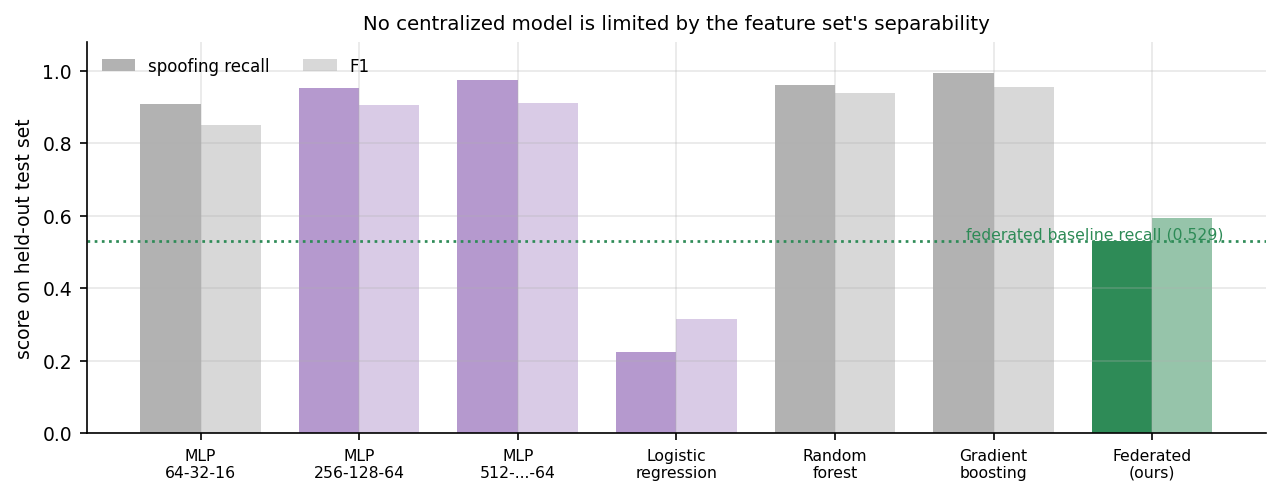
\includegraphics[width=3.4in]{figures/fig_detector_ceiling.png}
\caption{Centralized detector ceiling. Every centralized non-linear model far exceeds the federated baseline (dotted), so the weak spoofing recall reported throughout this paper reflects the federated training configuration rather than the separability of the feature set. This bounds what the security claims may assert: the paper supports removal of attacker-induced lift, not operational detection reliability.}
\label{fig:ceiling}
\end{figure}

\subsection{Computational Cost}
\label{subsec:cost}
The previous draft reported roughly $1.1\%$ server-side overhead. The review correctly identifies
that this used a sequential-simulation denominator that sums every client's training time, whereas
real UAV clients train in parallel and a round costs roughly the \emph{slowest} client. We withdraw
that figure as the headline number and report both denominators in Table~\ref{tab:cost}.

Measured on the ten-client configuration, the defense adds $34.0$~ms of server-side computation per
round. Against a sequential round of $3{,}449$~ms that is $0.98\%$; against a parallel round of
$999$~ms, bounded by the slowest client, it is $3.40\%$. The parallel figure is the honest one for a
deployment, and it is roughly three times larger than what we previously reported. FLTrust on the
same basis costs $168.3$~ms, or $16.9\%$ of a parallel round, because it trains a server model on
the root set every round; our probe is forward-pass only.

We also withdraw the claim that the defense remains practical as the fleet grows, because the
measurement does not support it. Server cost is linear in the number of clients ($19.3$, $34.0$,
$69.5$ and $139.1$~ms at $5$, $10$, $20$ and $40$ clients) while a parallel round stays roughly
constant, so the overhead \emph{fraction} rises with fleet size: $5.6\%$ at five clients, $9.6\%$ at
ten, $18.0\%$ at twenty and $34.9\%$ at forty. Cost is likewise linear in the probe count ($13.2$ to
$35.6$~ms from two to eight features) and grows only mildly with root-set size ($25.5$ to
$37.1$~ms from $600$ to $6{,}000$ rows). A large fleet would need the probe evaluated on a client
subsample or batched across rounds; we have not tested either, and make no claim about them.

\begin{table}[!t]
\renewcommand{\arraystretch}{1.25}
\caption{Server-Side Cost on Both Denominators (ten clients, mean of three timed rounds). A Sequential Round Sums Every Client's Training; a Parallel Round Is Bounded by the Slowest Client and Is the Realistic Denominator.}
\label{tab:cost}
\centering
\footnotesize
\setlength{\tabcolsep}{4pt}
\begin{tabular}{@{}l ccc@{}}
\toprule
\textbf{Defense} & \textbf{ms/round} & \textbf{\% sequential} & \textbf{\% parallel} \\
\midrule
Trust $+$ median (ours)       & $34.0$  & $0.98\%$ & $3.40\%$  \\
FLTrust \cite{cao2021fltrust} & $168.3$ & $4.88\%$ & $16.86\%$ \\
\bottomrule
\end{tabular}
\end{table}

\begin{figure}[!t]
\centering
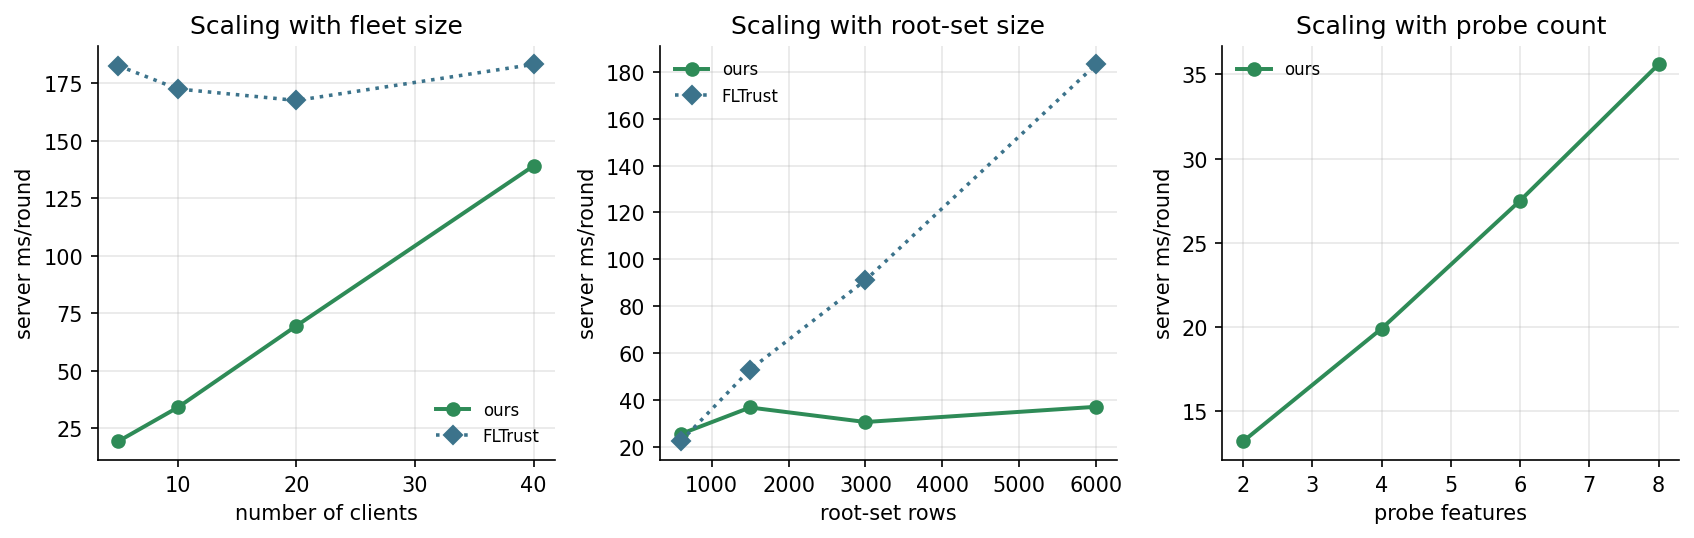
\includegraphics[width=3.45in]{figures/fig_overhead.png}
\caption{Measured server-side cost per round. Cost is linear in the number of clients and in the probe count, and nearly flat in root-set size. Because a parallel round's duration is set by the slowest client and does not grow with fleet size, the overhead \emph{fraction} rises with the fleet, reaching $34.9\%$ at forty clients. FLTrust is roughly five times more expensive at ten clients because it trains a server model each round.}
\label{fig:overhead}
\end{figure}

\section{Discussion}
The vulnerability this paper identifies is real and specific. Accuracy-weighted aggregation, adopted in recent UAV-FL work to reward good clients, is a second attack lever: inflation raises backdoor lift from $+0.2415$ to $+0.3036$, making the weighted rule worse than no weighting at all. A defense that never reads a self-reported metric is immune to that lever by construction rather than by tuning, and every rule we tested that ignores self-report is unaffected by inflation.

Beyond that, the revision's results are more qualified than the previous draft's, in three ways that we state directly rather than leave to be inferred.

\textit{The proposed defense is not uniquely necessary under IID data.} Multi-Krum reaches $+0.0061$ lift against our behavioral trust's $+0.0039$, a difference well inside the seed spread, at a twenty-seventh of the server cost. Where behavioral trust does separate itself is on assumptions and on outputs: Multi-Krum, trimmed mean and Krum must be told how many clients are compromised, and Section~\ref{subsec:fcount} shows Multi-Krum degrading from $+0.0061$ to $+0.2837$, essentially the undefended level, once the true count exceeds the configured $f$. The behavioral probe has no such parameter and stays flat across that range. It also produces a per-client trust value rather than a selection, so it names the compromised aircraft instead of merely excluding updates, which matters operationally.

\textit{The behavioral probe does not survive client heterogeneity, and that is the most important finding here.} Under even mild class-ratio skew the trust layer stops firing: attacker trust rises from $0.0001$ to uniform, detection falls from $100\%$ to single digits, and trust-only aggregation returns lift statistically indistinguishable from no defense at all. The mechanism is the robust scaling itself. Suspicion is measured in cohort MAD units, and heterogeneity inflates the MAD until a backdoored client's deficit no longer clears the dead-zone. Lowering the dead-zone recovers only part of the detection and costs honest false flags, so this is not a threshold that can simply be retuned. Any deployment on a genuinely heterogeneous fleet would need a suspicion statistic normalized per client rather than against a global cohort spread; designing and testing one is the clearest technical next step this work leaves open.

\textit{The median layer earns its place, but not where the previous draft claimed.} Under IID conditions its contribution is small and within noise, which is why we withdraw the claim that both layers are necessary in the evaluated setting. Its value appears exactly where the trust score fails: under skew it removes $0.173$ and $0.148$ of lift, an order of magnitude more than under IID. Coordinate-wise median is a backstop, and the realistic setting is the one that reveals why a backstop is worth keeping.

Two earlier claims are corrected outright. The overhead figure of $1.1\%$ used a sequential denominator; on the parallel denominator a deployment would actually experience, the same measurement is $3.40\%$, and because server cost is linear in the fleet while a parallel round is not, the fraction reaches $34.9\%$ at forty clients. We therefore withdraw any claim of large-fleet practicality. And the weak base detector is not a property of the dataset, as we previously suggested: centrally trained models reach $0.907$ to $0.993$ recall on the same features, so the limitation is our federated configuration.

What survives all of this is narrower than the original claim but better supported. Self-reported accuracy is an exploitable basis for aggregation weight; a coordinator that judges submitted models by their behavior on counterfactual spoofed samples closes that lever without needing to know the trigger feature, without needing to know how many clients are compromised, and while naming the ones that are; and under IID conditions it does so at no utility cost. The scope of that claim is IID or near-IID fleets, a single signal domain, and a detector weaker than the data supports.

\subsection*{Limitations}
Beyond the two corrections above, the following bound the results.

\textit{Heterogeneity.} The defense's headline advantage is demonstrated only under IID clients. Section~\ref{subsec:noniid} shows it does not extend to skewed fleets, which is the realistic case.

\textit{Dataset and domain.} The evaluation uses one public single-receiver software-defined-radio collection as a proxy for a fleet, because no public multi-UAV GPS spoofing dataset with labeled attacks exists. The attack and defense mechanisms do not refer to GPS specifically, but that is an argument, not evidence; a second independent signal domain would be the real test.

\textit{Detector strength.} At the paper's operating point an honest model already classifies $63.7\%$ of trigger-bearing samples as authentic. Driving backdoor lift to zero restores that baseline; it does not make the detector operationally reliable, and we do not claim it does.

\textit{Trigger scope.} The trigger-agnostic claim covers the probed feature set. Table~\ref{tab:features} shows the boundary sits an order of magnitude below the weakest probed feature, so a trigger hidden beneath it would carry little signal for the detector to exploit, but it is untested.

\textit{Statistical power and implementation.} Three seeds separate the attack effect from noise but cannot resolve sub-noise differences between neighboring defended variants, and we claim none. The sensitivity sweep varies one hyperparameter at a time, so the reported insensitivity is local. The FLTrust, Krum, Multi-Krum and trimmed-mean baselines are our own implementations on a shared harness, which is the right way to hold the setup fixed but means the comparison reflects our reading of each method.

\section{Conclusion}
We showed that accuracy-weighted federated aggregation, adopted in recent UAV-FL detection work to reward high-quality clients, is exploitable: two compromised UAV clients of ten can implant a stealthy GPS spoofing backdoor by poisoning a fraction of their data, scaling their updates, and inflating their reported accuracy, raising backdoor lift from $+0.2415$ to $+0.3036$ while clean accuracy falls by less than two points. We proposed a server-side behavioral-trust defense that never reads reported accuracy and does not need to know the trigger feature, and evaluated it against eight published aggregation rules on an identical pipeline.

Under IID clients the defense reduces attack-induced backdoor lift to a level statistically indistinguishable from the honest baseline ($-0.0265 \pm 0.0174$), flags both compromised clients in $100\%$ of client-rounds at a $0.3\%$ honest false-flag rate, generalizes across the discriminative feature set including a mixed trigger, remains effective against the tested defense-aware evasion objective, and adds $34.0$~ms of measured server-side computation per round for the evaluated ten-client configuration. It retains that protection when the number of compromised clients is unknown, a condition under which Multi-Krum and trimmed mean degrade to near-undefended performance, and it attributes the attack to specific aircraft rather than only excluding updates.

Its principal limitation is now measured rather than conjectured: under client class-ratio skew the behavioral probe stops firing, because suspicion measured in cohort median-absolute-deviation units is masked by the honest cohort's own variance, and the coordinate-wise median backstop carries what protection remains. A per-client suspicion statistic that does not depend on cohort spread, evaluation on a second signal domain, and a federated configuration that closes the gap to the centralized detector ceiling are the three concrete directions this work leaves open.

\section*{Artifact Availability}
All experiments are implemented in Python with PyTorch and scikit-learn and run on CPU. Every table and figure in this paper is produced by a notebook or script in the project repository and exported to a CSV or PNG, and the reported values are read from those exports rather than transcribed, so no figure or table can disagree with the run that produced it. The FLTrust comparison of Section~\ref{subsec:benchmark} and the feature-separability table of Section~\ref{subsec:data} are each produced by a single self-contained script that re-derives the data split from the same fixed seed, so both can be reproduced with one command and without running the notebooks. Given the fixed data seed, the federated runs are deterministic and reproduce bit-identically between executions on the same machine. The dataset is publicly available \cite{aissou2022dataset}.

\section*{Acknowledgment}
The authors thank Dr. Khalid Hasan for advising this capstone project at James Madison University.

\bibliographystyle{IEEEtran}
\bibliography{references}

\end{document}
